\subsection{KMeans Algorithm}
%----------------------------------------------------
% Alternative 1: Algorithmic Setup
\begin{algorithm}[H]
\caption{KMeans Clustering Algorithm}
\label{alg:KMeans}
\begin{algorithmic}[1]
\State \textbf{Input:} Embedding vectors $\{\mathbf{e}^1, \mathbf{e}^2, \ldots, \mathbf{e}^{N}\}$, number of clusters $k$
\State \textbf{Output:} Cluster assignments $\{\D_1, \D_2, \ldots, \D_k\}$, centroids $\{\mathbf{c}_1, \mathbf{c}_2, \ldots, \mathbf{c}_k\}$

\State \textbf{Initialize} centroids $\{\mathbf{c}_1, \mathbf{c}_2, \ldots, \mathbf{c}_k\}$ randomly

\Repeat
    \State \underline{\textit{Assignment Step:}}
    \For{each vector $\mathbf{e}^i$}
        \State Assign $\mathbf{e}^i$ to the nearest centroid:
        \[
        g = \arg \min_{\ell\in\{1,...,k\}} \|\mathbf{e}^i - \mathbf{c}_{\ell}\|_{2}^2
        \]
        \State Update cluster assignments: $\D_{g} \leftarrow \D_{g} \cup \{i\}$
    \EndFor

    \State \underline{\textit{Update Step:}}
    \For{each cluster $\D_g$}
        \State Recalculate centroid $\mathbf{c}_g$:
        \[
        \mathbf{c}_g = \frac{1}{|\D_g|} \sum_{i \in \D_g} \mathbf{e}^i
        \]
    \EndFor
\Until{cluster assignments no longer change}

\State \textbf{Return} cluster assignments $\{\D_1, \D_2, \ldots, \D_k\}$ and centroids $\{\mathbf{c}_1, \mathbf{c}_2, \ldots, \mathbf{c}_k\}$

\end{algorithmic}
\end{algorithm}

%----------------------------------------------------
% Alternative 2: More organized setup
%\section*{KMeans Clustering Algorithm}

\subsection*{Inputs}
\begin{itemize}
    \item Embedding vectors: $\{\mathbf{e}^1, \mathbf{e}^2, \ldots, \mathbf{e}^{N_{tr}}\}$
    \item Number of clusters: $k$
\end{itemize}

\subsection*{Outputs}
\begin{itemize}
    \item Cluster assignments: $\{C_1, C_2, \ldots, C_k\}$
    \item Centroids: $\{\mathbf{c}_1, \mathbf{c}_2, \ldots, \mathbf{c}_k\}$
\end{itemize}

\subsection*{Algorithm}
\begin{enumerate}
    \item \textbf{Initialize} centroids $\{\mathbf{c}_1, \mathbf{c}_2, \ldots, \mathbf{c}_k\}$ randomly.
    \item \textbf{Repeat until convergence:}
    \begin{enumerate}
        \item \textbf{Assignment Step:}
        \[
        C_j = \left\{ \mathbf{e}^i \mid j = \arg \min_{l} \|\mathbf{e}^i - \mathbf{c}_l\|^2, \quad l = 1, 2, \ldots, k \right\}
        \]
        \item \textbf{Update Step:}
        \[
        \mathbf{c}_j = \frac{1}{|C_j|} \sum_{\mathbf{e}^i \in C_j} \mathbf{e}^i, \quad \forall j = 1, 2, \ldots, k
        \]
    \end{enumerate}
    \item \textbf{Convergence Criterion:} Repeat steps 2(a) and 2(b) until the cluster assignments do not change, i.e.,
    \[
    C_j^{(t+1)} = C_j^{(t)}, \quad \forall j = 1, 2, \ldots, k
    \]
    where $t$ denotes the iteration number.
\end{enumerate}

\subsection*{Objective}
The KMeans algorithm aims to minimize the within-cluster sum of squares (WCSS):
\[
\min_{C, \mathbf{c}} \sum_{j=1}^k \sum_{\mathbf{e}^i \in C_j} \|\mathbf{e}^i - \mathbf{c}_j\|^2
\]


%----------------------------------------------------

\newpage
\subsection{Hyperparameter Choice}
Our hyperparameters are $L$ and $\theta$. Recall that $L$ denotes the number of trading days over which we hold the positions in the beta-neutral strategy, while $\theta$ represents the upper bound on each side (long and short) for the amount of clusters we select for the trading strategy. The specific choice of hyperparameters we made for the results presented in the paper were:
\begin{align*}
L &= 4
\\
\theta &= \integer{0.5k}
\end{align*}
where $k$ represents the number of clusters (26 for KMeans clustering, and 20 for LLM clustering). This choice is not arbitrary nor opportunistic. Instead, it results from the maximization of the Sharpe Ratio of the portfolio in the train and validation samples for both KMeans and LLM clustering. This choice procedure is completely based on \textit{in-sample} criteria and it prevents lookahead bias. The justification for such choices is made below.

\subsubsection{KMeans Clustering}

In \cref{fig:KMeans_hyperparameter_justification_L} we can see that a choice of $L=4$ in the training and validation splits generates the most stable Sharpe Ratio. Namely, In the train set (\cref{fig:K_hyp_1}), it makes more sense to choose low values of $L$ (less than 4) to maximize the $SR$. However, in the validation set (\cref{fig:K_hyp_2}), it makes more sense to choose higher values of $L$. The choice of $L=4$ stands as a middle ground between this contradiction, generating a stable choice and a stable profile of earnings in sample.

%----------------------------------------------------
\inserthere{fig:KMeans_hyperparameter_justification_L}
\begin{figure}[H]
  \caption{Sharpe Ratios in the train and validation splits as a function of $L$ (KMeans)}
  \centering
  
  \begin{subfigure}[b]{0.46\textwidth}
    \centering
    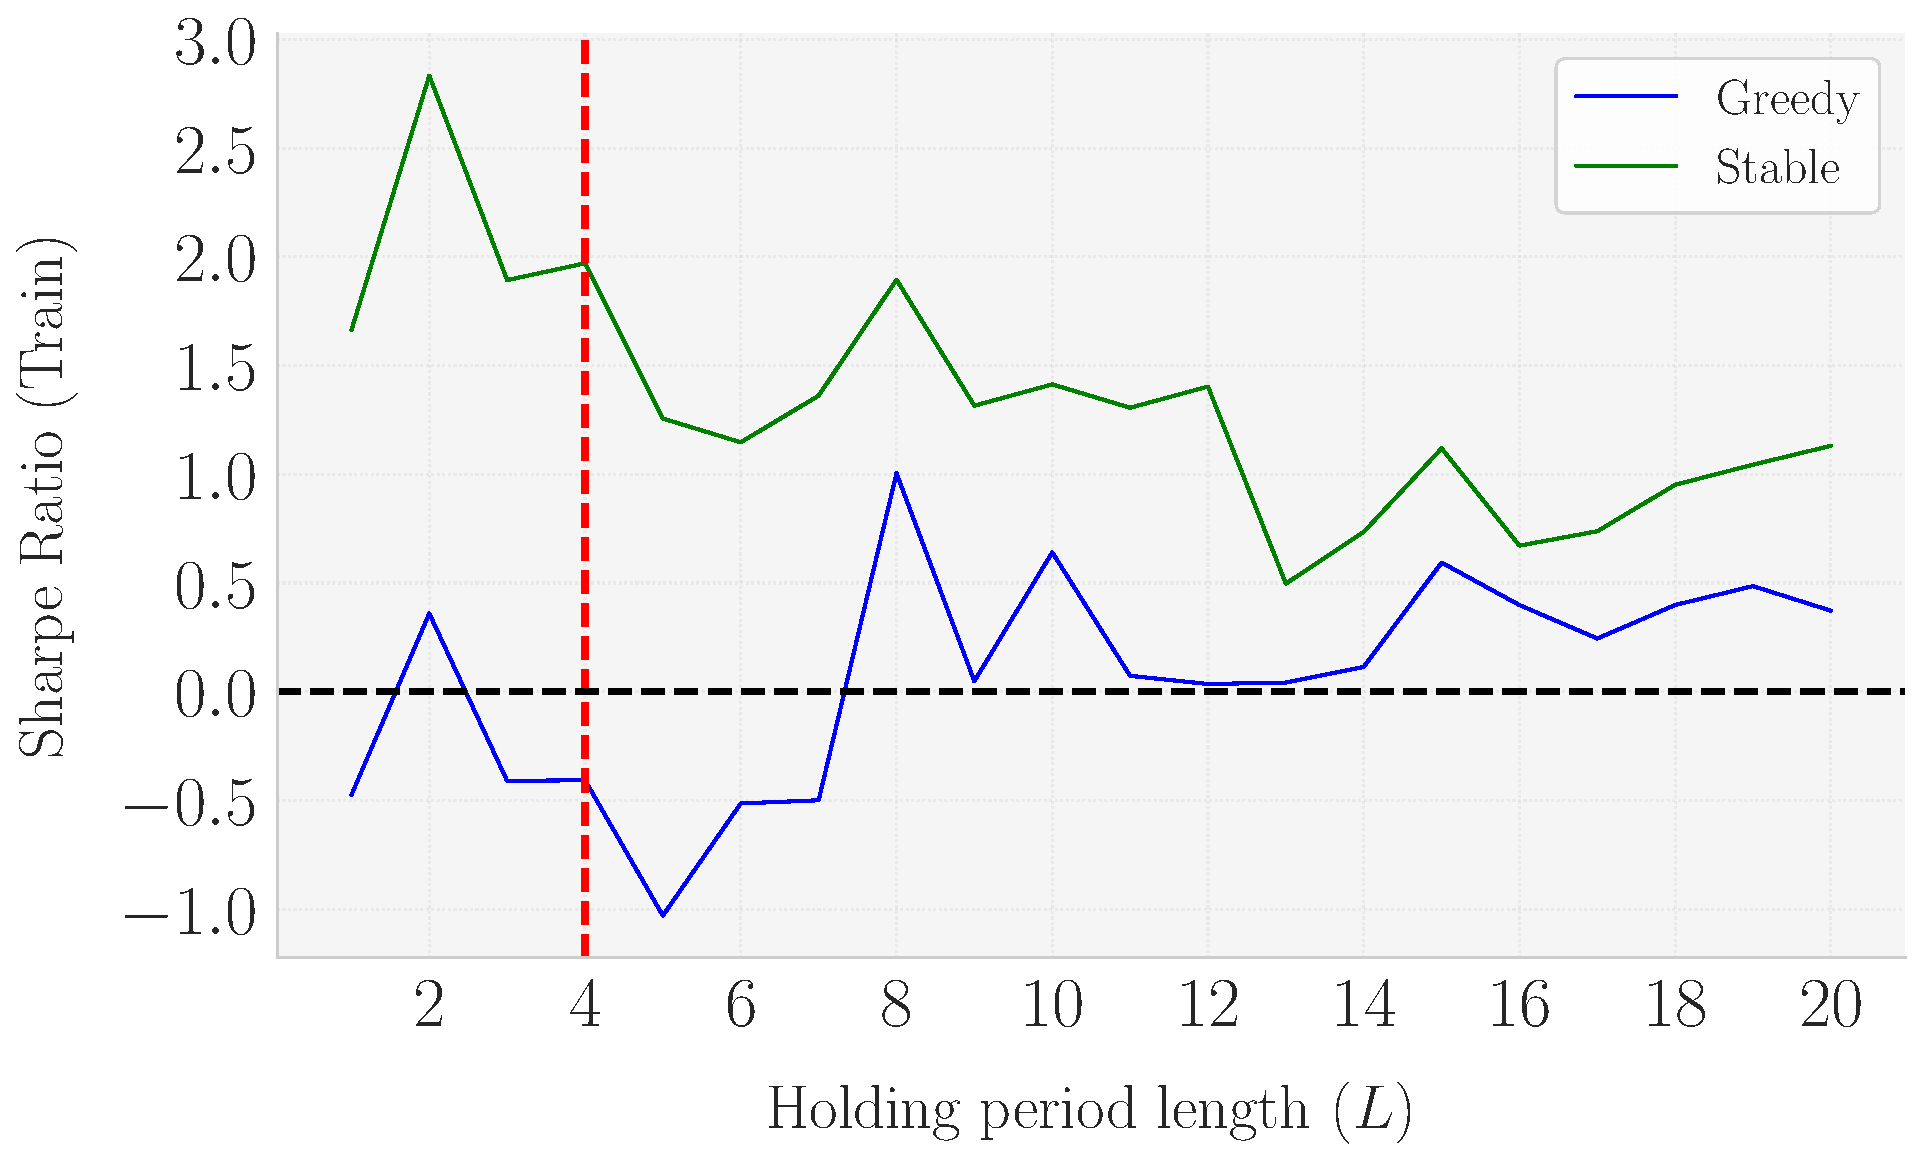
\includegraphics[width=\textwidth]{/Users/jesusvillotamiranda/Library/CloudStorage/OneDrive-UniversidaddeLaRioja/CEMFI/__MSc__/__Second_year__/6th_Term/MasterThesis/__Output/KMeans_RobustnessCheck_SR_Train_Set_vs_L_[Change_L].pdf}
    \caption{Plot of $SR^{\mathcal P^{tr}}(L)$ over a grid of $L$}
    \label{fig:K_hyp_1}
  \end{subfigure}
  \hspace{0.05\textwidth} % Add horizontal space between the subfigures
  \begin{subfigure}[b]{0.46\textwidth}
    \centering
    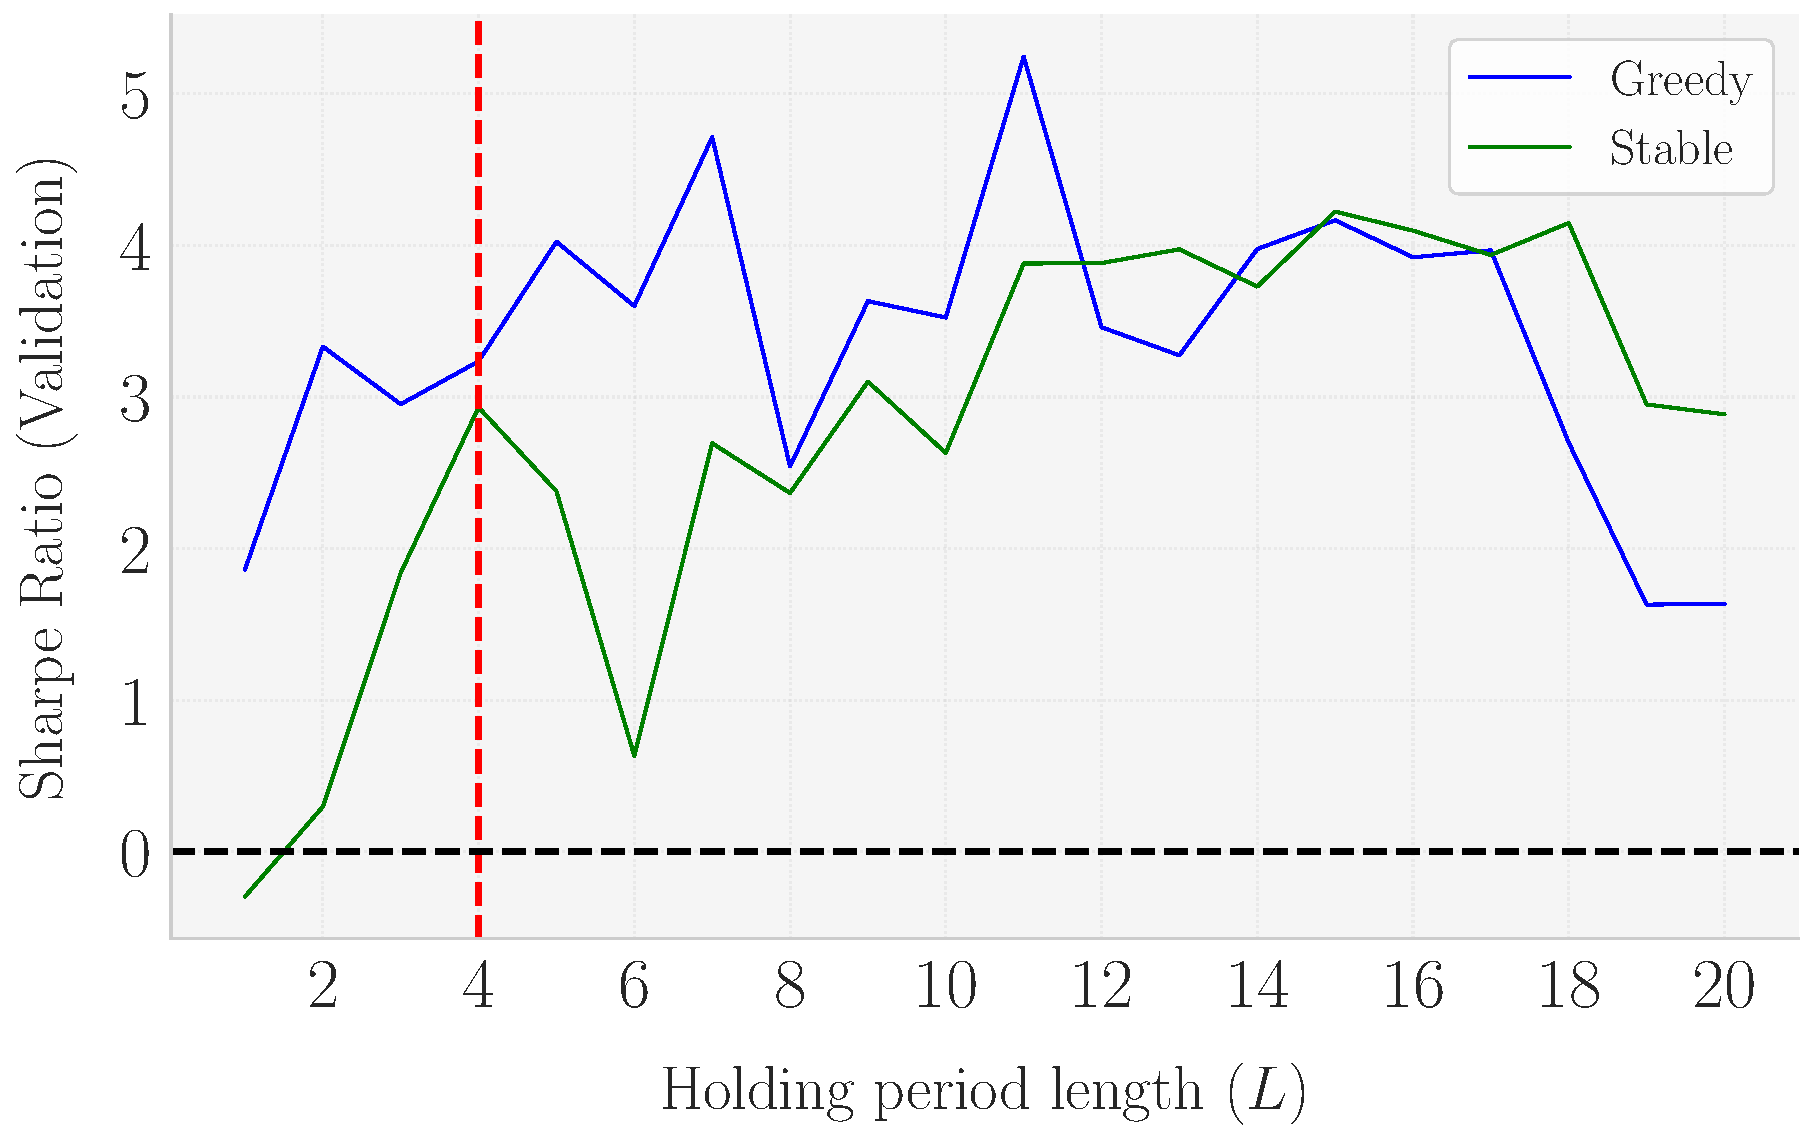
\includegraphics[width=\textwidth]{/Users/jesusvillotamiranda/Library/CloudStorage/OneDrive-UniversidaddeLaRioja/CEMFI/__MSc__/__Second_year__/6th_Term/MasterThesis/__Output/KMeans_RobustnessCheck_SR_Validation_Set_vs_L_[Change_L].pdf}
    \caption{Plot of $SR^{\mathcal P^{val}}(L)$ over a grid of $L$}
    \label{fig:K_hyp_2}
  \end{subfigure}  
  \label{fig:KMeans_hyperparameter_justification_L}
\end{figure}
%----------------------------------------------------

On the other hand, the choice of $\theta=\integer{0.5\cd 26}=13$ is a choice that pursues stability in the Sharpe Ratio of the train and validation portfolios. As we can see from \cref{fig:KMeans_hyperparameter_justification_theta}, the Sharpe Ratios tend to converge to the highest and most stable value when we choose the highest possible value of $\theta$. 

 %----------------------------------------------------
\inserthere{fig:KMeans_hyperparameter_justification_theta}
\begin{figure}[H]
  \caption{Sharpe Ratios in the train and validation splits as a function of $\theta$ (KMeans)}
  \centering
    \begin{subfigure}[b]{0.46\textwidth}
    \centering
    \includegraphics[width=\textwidth]{/Users/jesusvillotamiranda/Library/CloudStorage/OneDrive-UniversidaddeLaRioja/CEMFI/__MSc__/__Second_year__/6th_Term/MasterThesis/__Output/KMeans_RobustnessCheck_SR_Train_Set_vs_theta_[Change_theta].pdf}
    \caption{Plot of $SR^{\mathcal P^{tr}}(\theta)$ over a grid of $\theta$}
    \label{fig:K_hyp_3}
  \end{subfigure}
  \hspace{0.05\textwidth} % Add horizontal space between the subfigures
  \begin{subfigure}[b]{0.46\textwidth}
    \centering
    \includegraphics[width=\textwidth]{/Users/jesusvillotamiranda/Library/CloudStorage/OneDrive-UniversidaddeLaRioja/CEMFI/__MSc__/__Second_year__/6th_Term/MasterThesis/__Output/KMeans_RobustnessCheck_SR_Validation_Set_vs_theta_[Change_theta].pdf}
    \caption{Plot of $SR^{\mathcal P^{val}}(\theta)$ over a grid of $\theta$}
    \label{fig:K_hyp_4}
  \end{subfigure}
  \label{fig:KMeans_hyperparameter_justification_theta}
\end{figure}
%----------------------------------------------------


\subsubsection{LLM Clustering}
Following a similar logic as below, the choice of $L=4$ sets a consensus between the maximization of $SR^{\mathcal P^{tr}}$ and $SR^{\mathcal P^{val}}$. That is, maximizing $SR^{\mathcal P^{tr}}$ requires lower holding period lengths (the maximizer is $L=4$), while maximizing $SR^{\mathcal P^{val}}$ requires increasing the window length. Among this contradiction, $L=4$ standing as a perfect choice to balance the maximization requirements in both samples, generating a stable choice for the holding period window length.

%----------------------------------------------------
\inserthere{fig:LLM_hyperparameter_justification_L}
\begin{figure}[H]
  \caption{Sharpe Ratios in the train and validation splits as a function of hyperparameters (LLM)}
  \centering
  
  \begin{subfigure}[b]{0.46\textwidth}
    \centering
    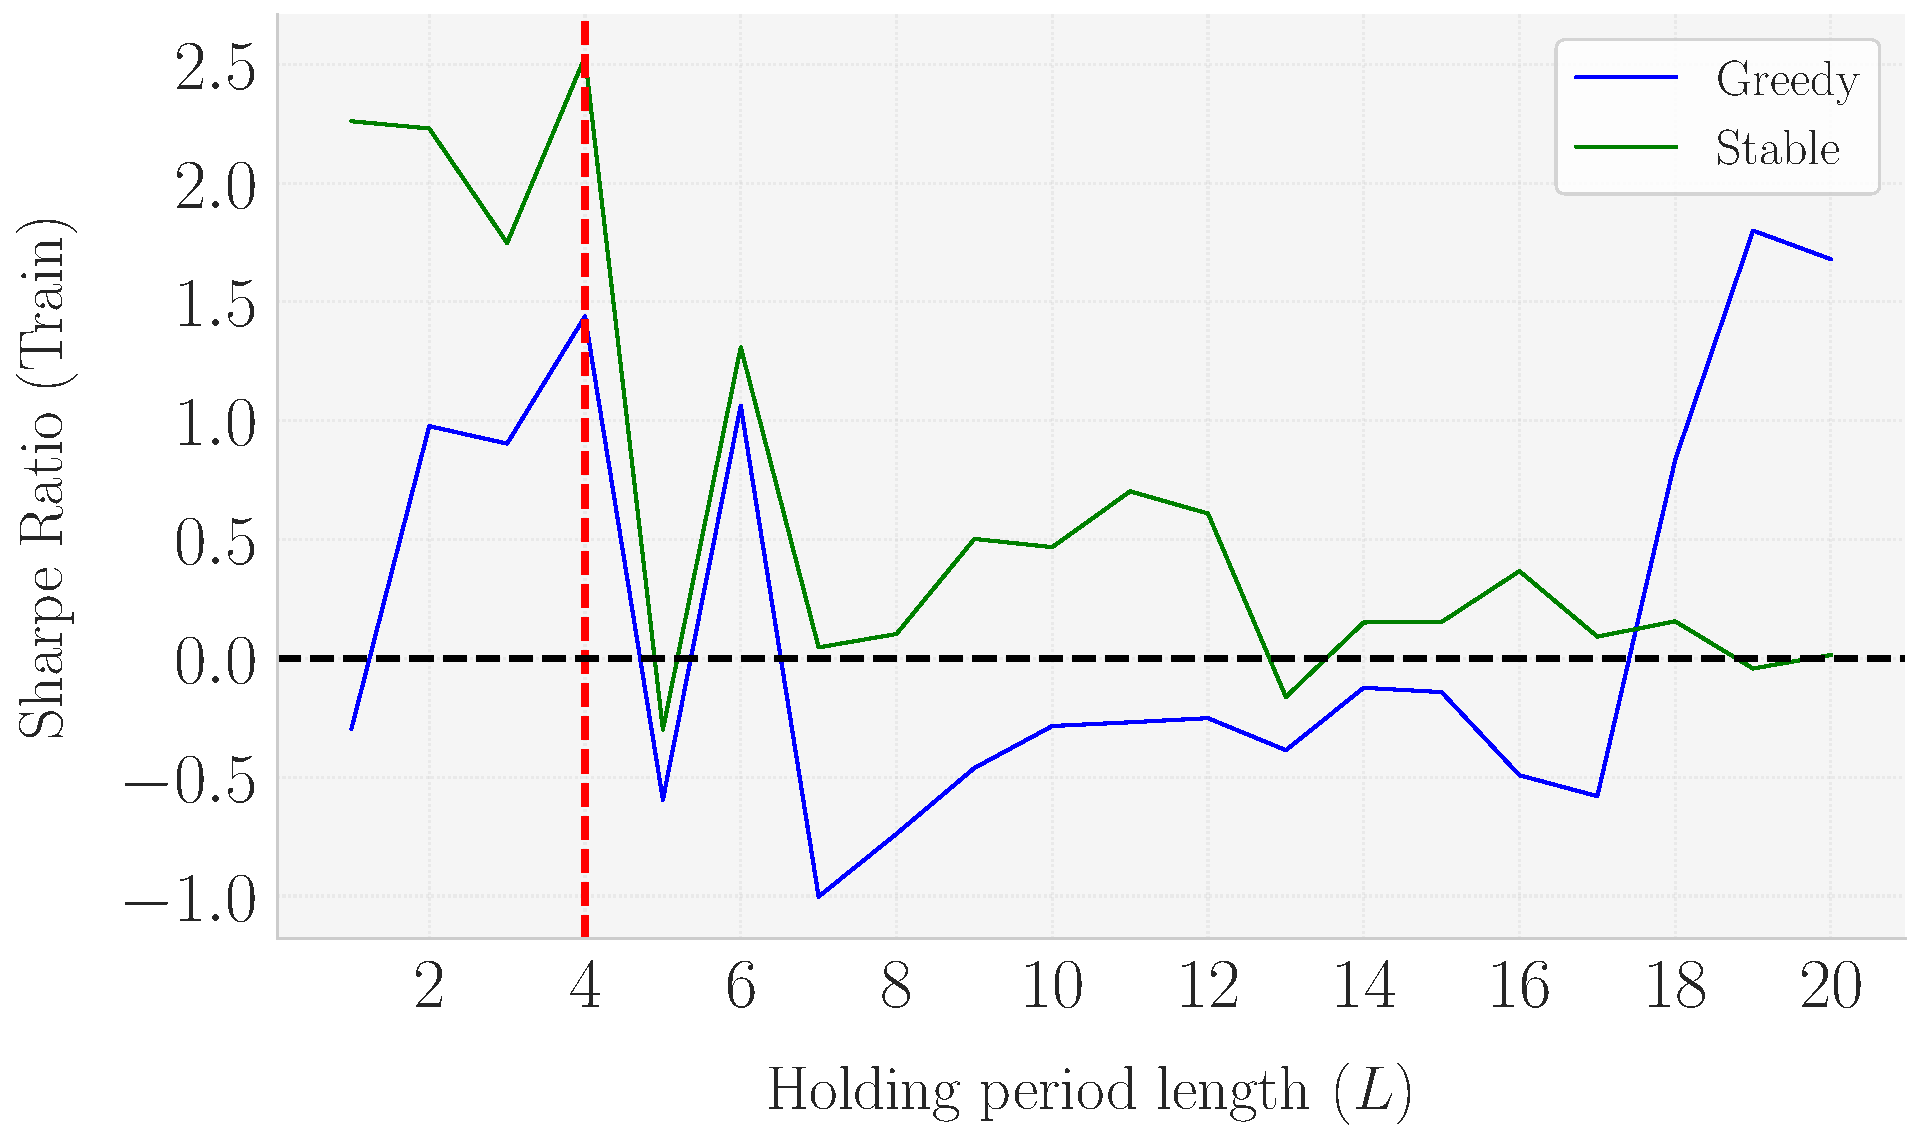
\includegraphics[width=\textwidth]{/Users/jesusvillotamiranda/Library/CloudStorage/OneDrive-UniversidaddeLaRioja/CEMFI/__MSc__/__Second_year__/6th_Term/MasterThesis/__Output/LLAMA_RobustnessCheck_SR_Train_Set_vs_L_[Change_L].pdf}
    \caption{Plot of $SR^{\mathcal P^{tr}}(L)$ over a grid of $L$}
    \label{fig:LLM_hyp_1}
    
  \end{subfigure}
  \hspace{0.05\textwidth} % Add horizontal space between the subfigures
  \begin{subfigure}[b]{0.46\textwidth}
    \centering
    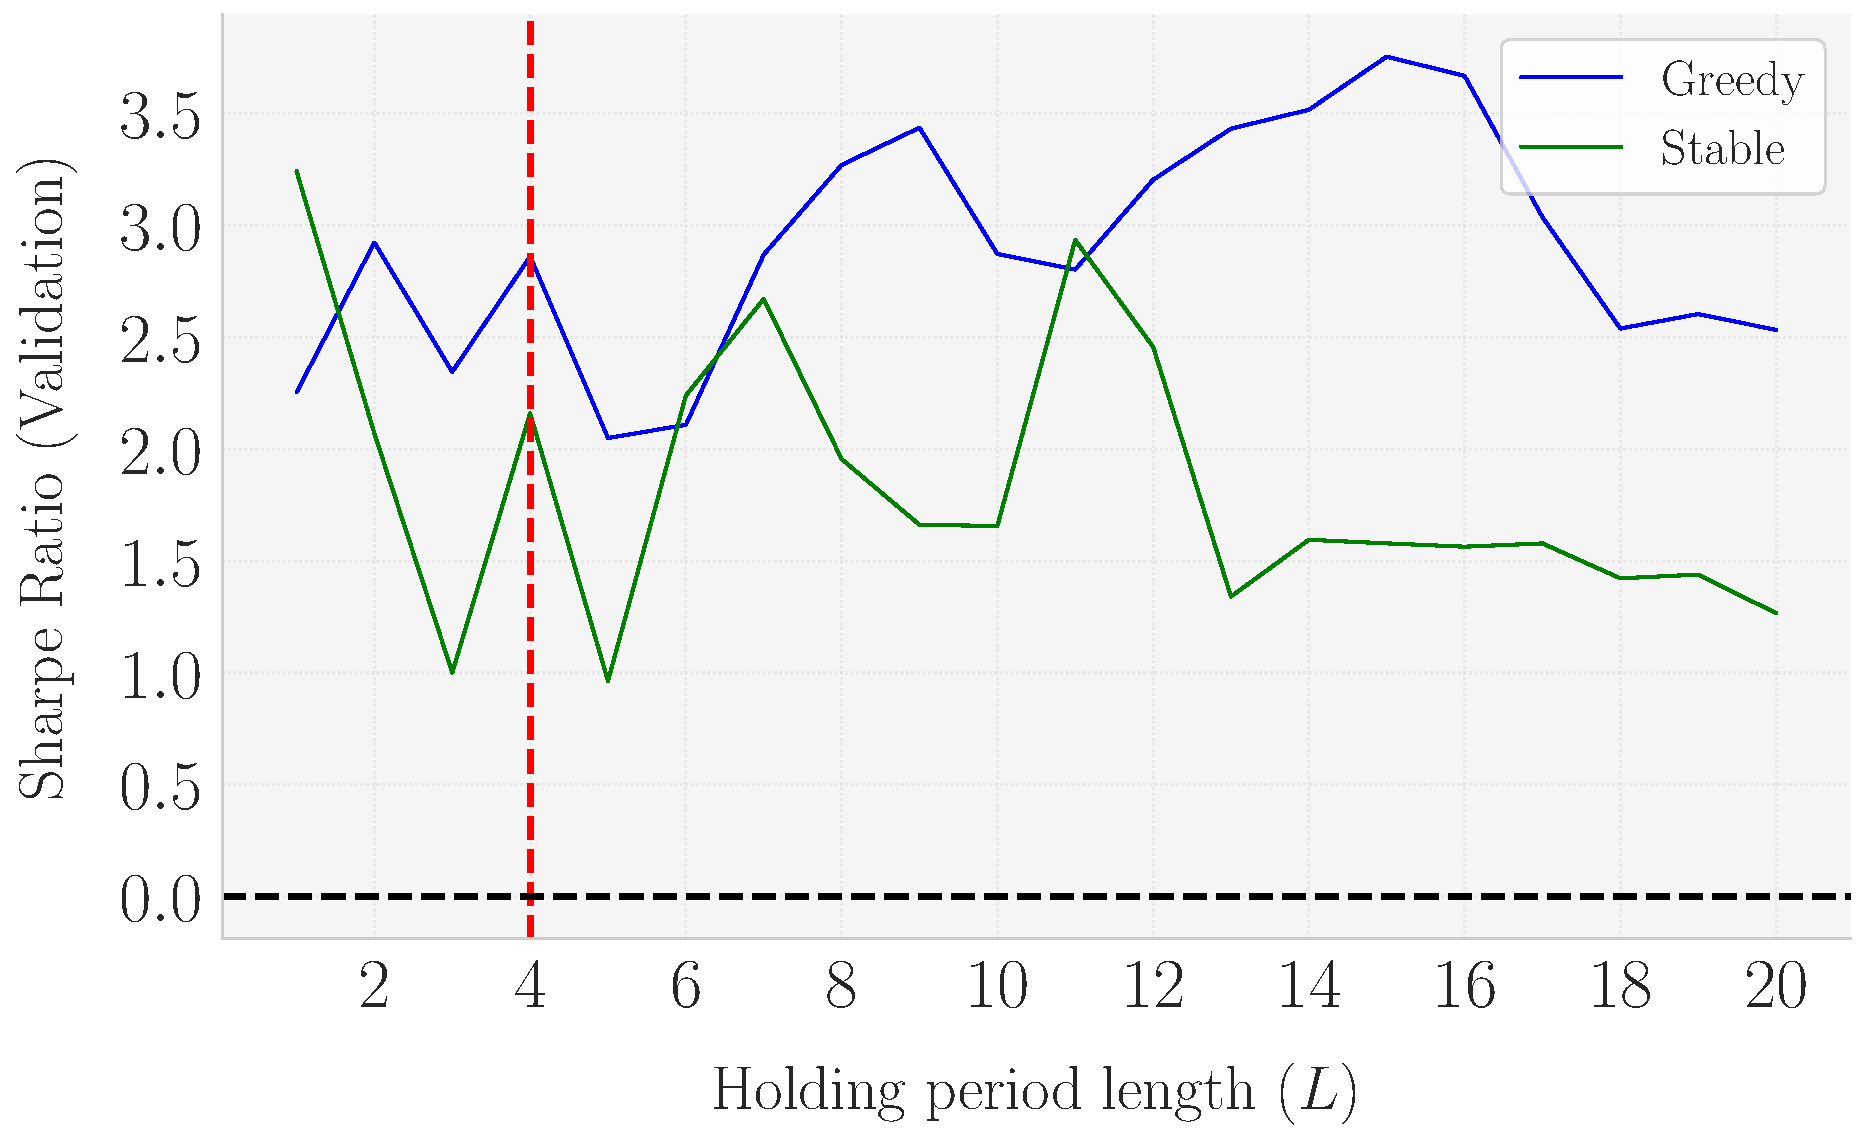
\includegraphics[width=\textwidth]{/Users/jesusvillotamiranda/Library/CloudStorage/OneDrive-UniversidaddeLaRioja/CEMFI/__MSc__/__Second_year__/6th_Term/MasterThesis/__Output/LLAMA_RobustnessCheck_SR_Validation_Set_vs_L_[Change_L].pdf}
    \caption{Plot of $SR^{\mathcal P^{val}}(L)$ over a grid of $L$}
    \label{fig:LLM_hyp_2}
  \end{subfigure}
  
  \label{fig:LLM_hyperparameter_justification_L}
\end{figure}
%----------------------------------------------------

Finally, the same conclusion as in KMeans applies here. By selecting $\theta=\integer{0.5\cd 20}=10$, we get a stable Sharpe Ratio. Even though we observe that $SR^{\mathcal P^{tr}}(L)$ falls momentarily at $\theta=10$ for the Greedy algorithm, it still constitutes a good choice. Conversely, at $\theta=10$ the greedy algorithm sees a jump in $SR^{\mathcal P^{val}}(L)$. All in all, we can easily conclude that $\theta=\integer{0.5k}$ arises as a good hyperpamrameter choice also for LLM clustering.
%----------------------------------------------------
\inserthere{fig:LLM_hyperparameter_justification_theta}
\begin{figure}[H]
\caption{Sharpe Ratios in the train and validation splits as a function of $\theta$ (LLM)}
  \centering

    \begin{subfigure}[b]{0.46\textwidth}
    \centering
    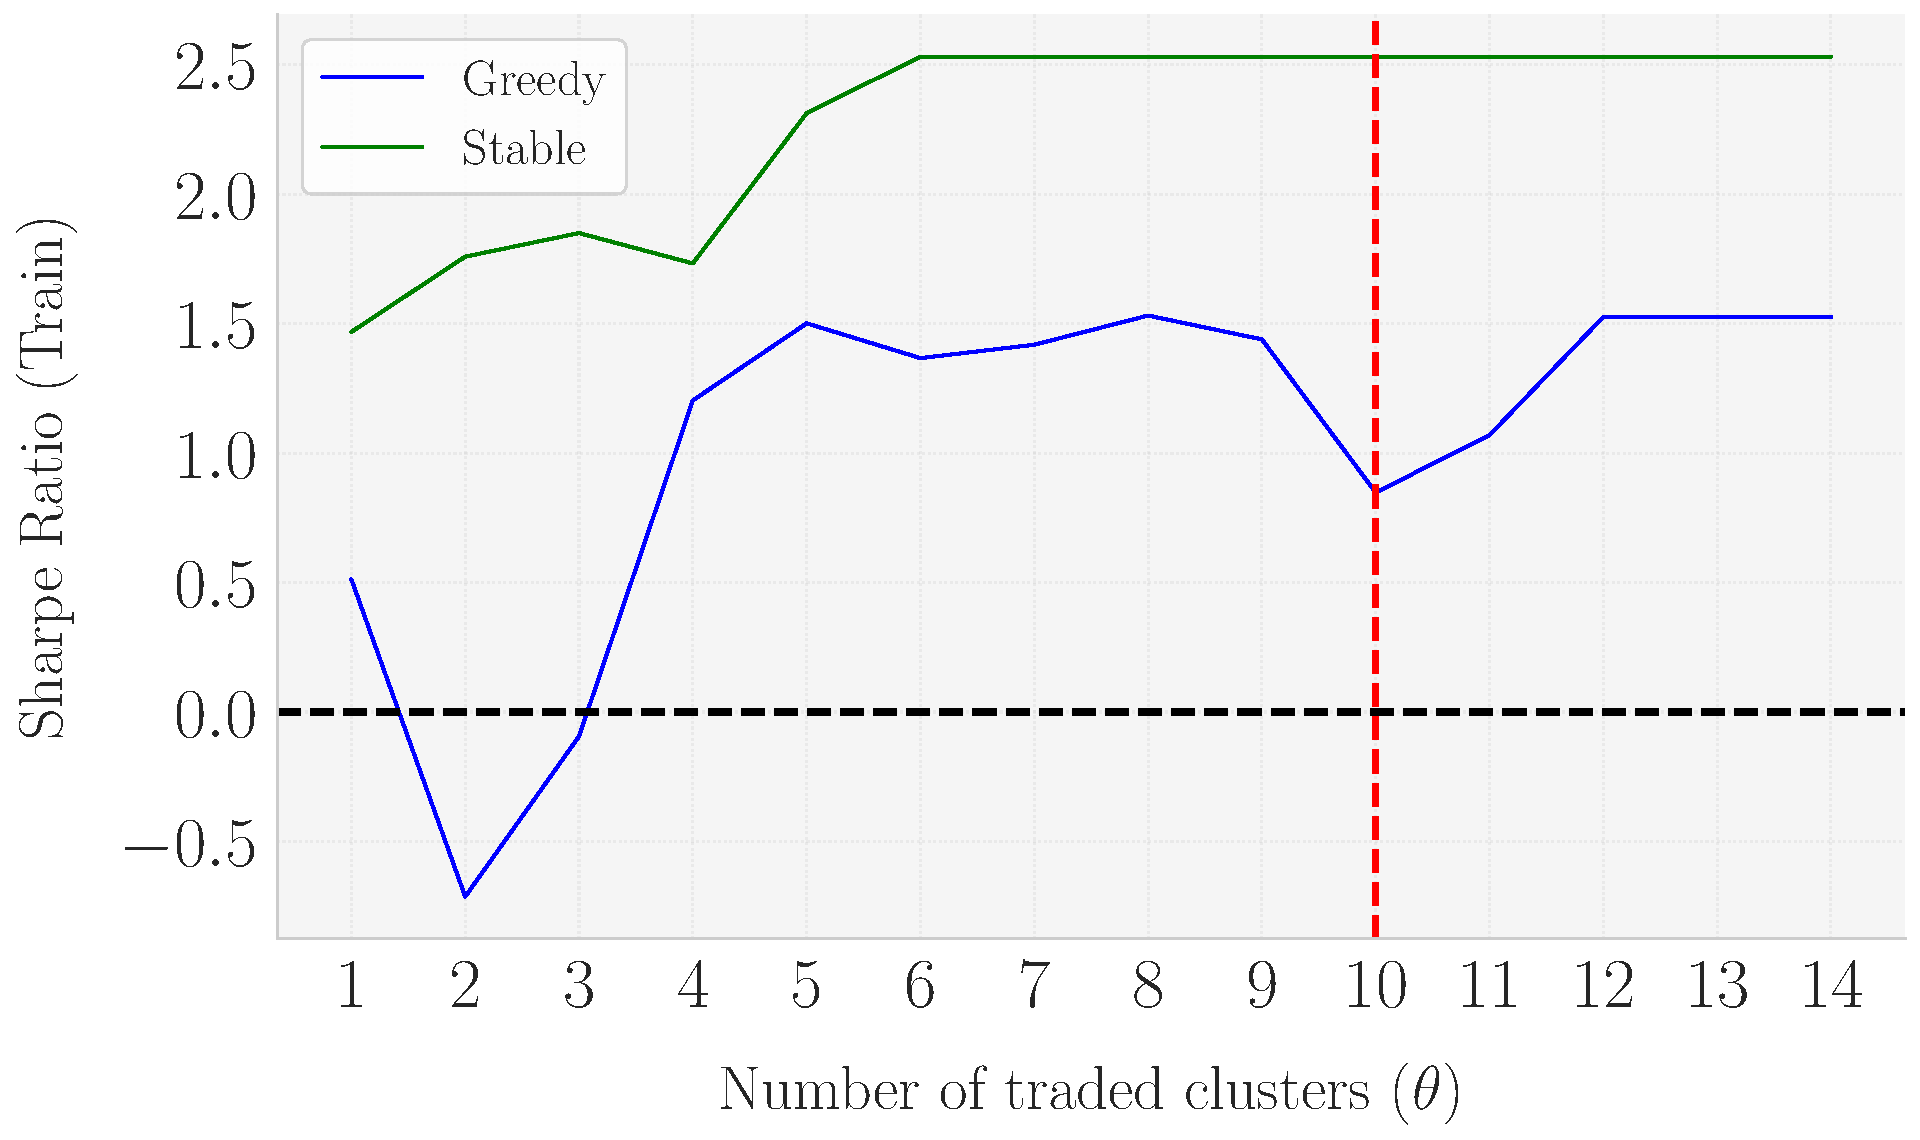
\includegraphics[width=\textwidth]{/Users/jesusvillotamiranda/Library/CloudStorage/OneDrive-UniversidaddeLaRioja/CEMFI/__MSc__/__Second_year__/6th_Term/MasterThesis/__Output/LLAMA_RobustnessCheck_SR_Train_Set_vs_Theta_[Change_theta].pdf}
    \caption{Plot of $SR^{\mathcal P^{tr}}(\theta)$ over a grid of $\theta$}
    \label{fig:LLM_hyp_3}
  \end{subfigure}
  \hspace{0.05\textwidth} % Add horizontal space between the subfigures
  \begin{subfigure}[b]{0.46\textwidth}
    \centering
    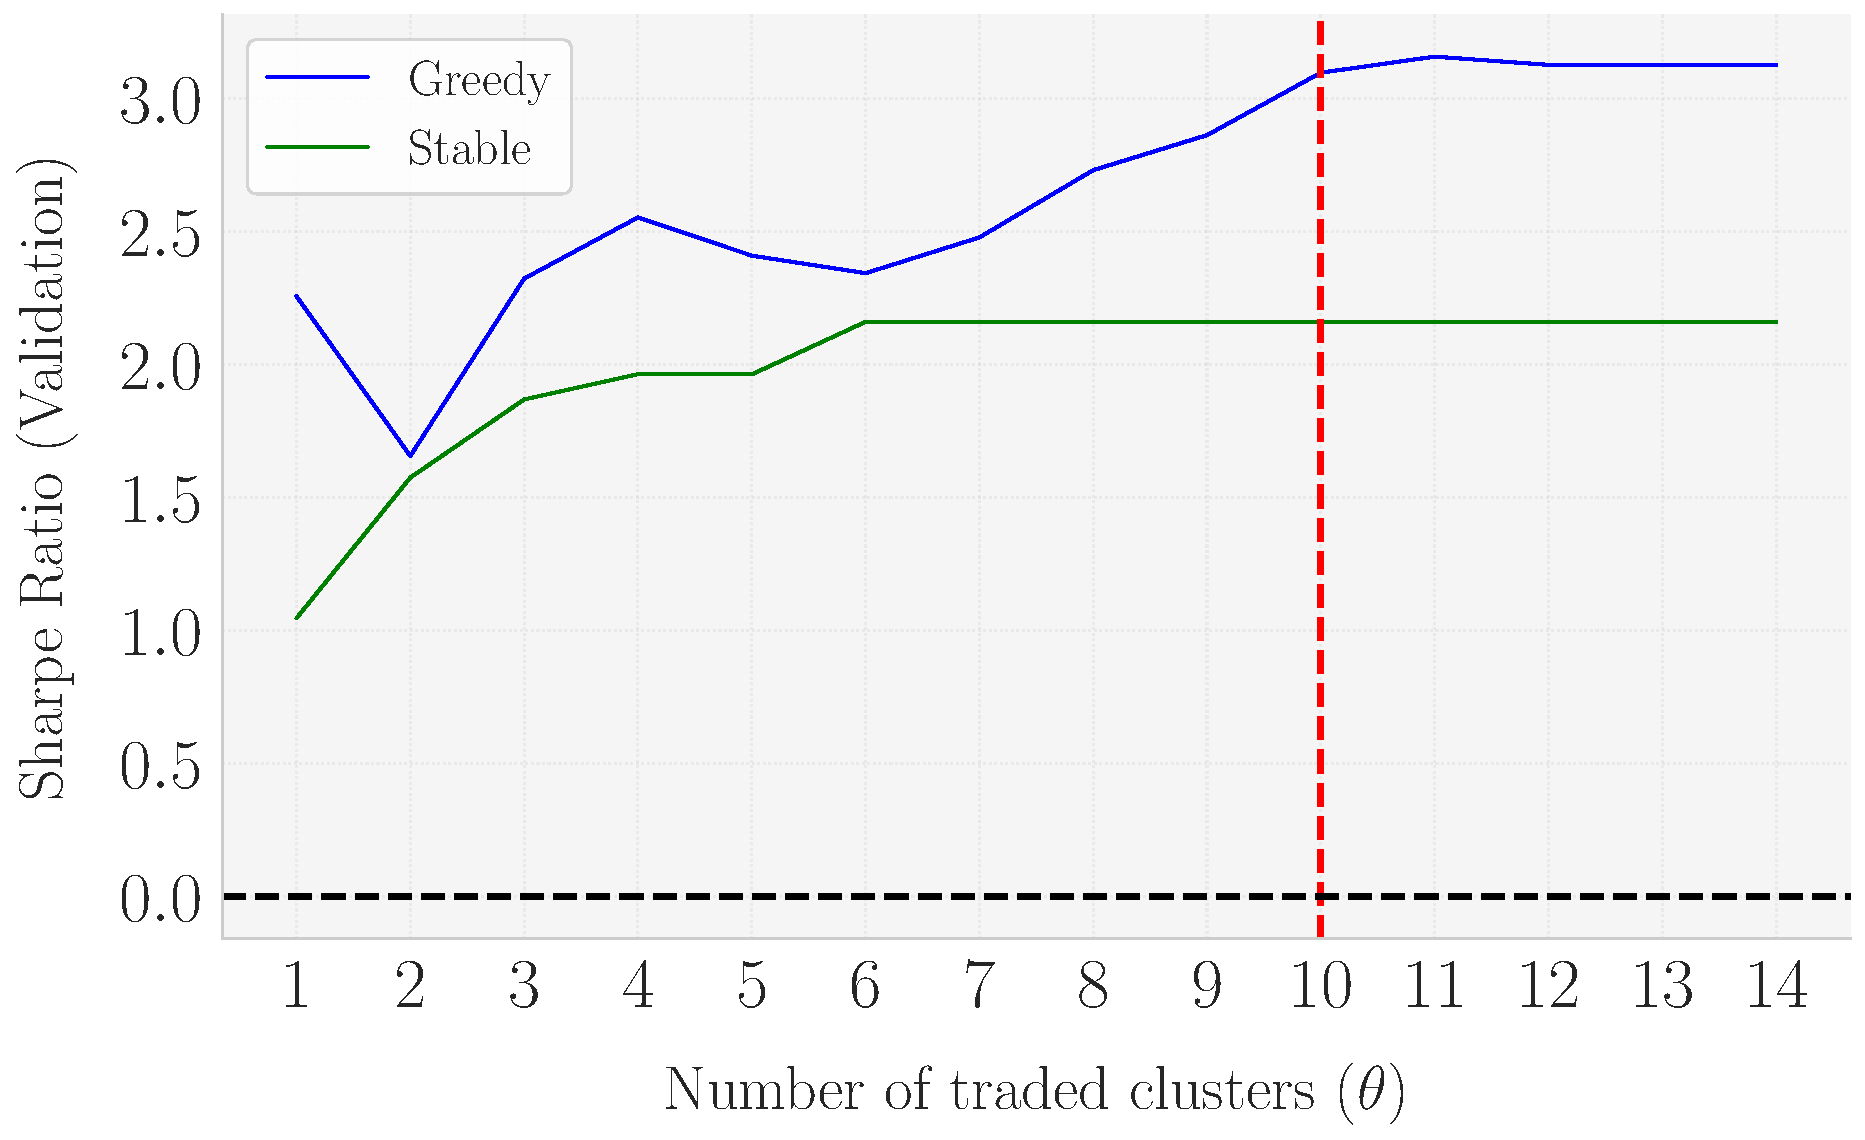
\includegraphics[width=\textwidth]{/Users/jesusvillotamiranda/Library/CloudStorage/OneDrive-UniversidaddeLaRioja/CEMFI/__MSc__/__Second_year__/6th_Term/MasterThesis/__Output/LLAMA_RobustnessCheck_SR_Validation_Set_vs_Theta_[Change_theta].pdf}
    \caption{Plot of $SR^{\mathcal P^{val}}(\theta)$ over a grid of $\theta$}
    \label{fig:LLM_hyp_4}
  \end{subfigure}

\label{fig:LLM_hyperparameter_justification_theta}
\end{figure}
%----------------------------------------------------




\newpage
%%%%%%%%%%%%%%%%%%%%%%%%%%%%%%%%%%%%%%%%%%%%%%%%%%%%%
\subsection{Optimal Cluster Selection Algorithms}
%%%%%%%%%%%%%%%%%%%%%%%%%%%%%%%%%%%%%%%%%%%%%%%%%%%%%
%----------------------------------------------------
\begin{algorithm}
\caption{
\textsc{Greedy Selection} 
~|~
{{Top average Sharpe Ratio in Validation Set}}
}
%%%%%%%%%%%%%%%%%%%%%%%%%%%%%%%%%%%%%%%%%%%%%%%%%%%%%
\label{alg:greedy_selection}
%%%%%%%%%%%%%%%%%%%%%%%%%%%%%%%%%%%%%%%%%%%%%%%%%%%%%
\begin{algorithmic}[1]
\mx 
\State \textbf{Input:} Set of clusters $\mathcal{G} = \{1, 2, \ldots, k^*\}$, Sharpe Ratios in the validation sample $\{SR_L^{(i,j)}\}_{(i,j)\in \mathcal B^{val}}$, maximum number of traded clusters $\theta\in\mathbb{N}$ (usually, $\theta\propto k^*)$

\mx 
\State \textbf{Output:} Set of long-traded clusters $\mathcal{G}_{\theta}^{+}$ and set of short-traded clusters $\mathcal{G}_{\theta}^{-}$
%----------------------------------------------------
%\Statex
\vspace{0.4cm}
\Statex \underline{\textit{Step \#1: Compute Cluster Average Sharpe Ratios in Validation Set}}
\For{each $g \in \mathcal{G}$}
    \State Compute average Sharpe Ratio ~
$
\overline{S R}_g^{val} \leftarrow \frac{1}{|\mathcal{B}_g^{val} |} \sum_{(i,j) \in \mathcal{B}_g^{val}} S R_{{{L}}}^{(i,j)}
$
\EndFor
%----------------------------------------------------
%\Statex
\vspace{0.4cm}
\Statex \underline{\textit{Step \#2: Identify Positive and Negative Sharpe Ratio Clusters}}
\State Define $\mathcal{G}_{SR^+}^{val} \leftarrow \{ g \in \mathcal{G} \mid \overline{SR}_g^{val} > 0 \}$
\State Define $\mathcal{G}_{SR^-}^{val} \leftarrow \{ g \in \mathcal{G} \mid \overline{SR}_g^{val} < 0 \}$
%----------------------------------------------------
\vspace{0.4cm}
\Statex \underline{\textit{Step \#3: Rank Clusters by Average Sharpe Ratio in the Validation Set}}
\For{each $g \in \mathcal{G}$}
	\State Rank the average Sharpe Ratio~~
$
\mathfrak{R}_g^{val} \leftarrow  \sum_{h \in \mathcal{G}} 
\mathbf{1}\1{
\overline{S R}_h^{val} \geq \overline{S R}_g^{val} 
}
$
\EndFor
%\State Sort clusters in descending order of $\overline{SR}_g^{val}$
%%\State
%$$\overline{SR}_{\varkappa_1}^{val} \geq \overline{SR}_{\varkappa_2}^{val} \geq \ldots \geq \overline{SR}_{\varkappa_{k^*}}^{val}$$
%----------------------------------------------------
%\Statex
\vspace{0.4cm}
\Statex \underline{\textit{Step \#4: Select Top $\theta$ Clusters}}
\State Define $\theta^+ \leftarrow \min(\theta, |\mathcal{G}_{SR^+}^{val}|)$
;~~
$\mathcal{G}_{\theta}^{+} \leftarrow \{ g\in\G \mid 1 \leq \mathfrak{R}_g^{val} \leq \theta^+ \}$
%\State 

\State Define $\theta^- \leftarrow \min(\theta, |\mathcal{G}_{SR^-}^{val}|)$
;~~
%\State 
 $\mathcal{G}_{\theta}^{-} \leftarrow \{ g \in\G \mid k^* - \theta^- < \mathfrak{R}_g^{val} \leq k^* \}$
%----------------------------------------------------
%\Statex
\vspace{0.5cm}
\State \textbf{Return} Long-traded clusters $\mathcal{G}_{\theta}^{+}$, Short-traded clusters $\mathcal{G}_{\theta}^{-}$

\end{algorithmic}
\end{algorithm}


%
%\begin{algorithm}[H]
%\caption{Greedy Selection of Clusters Based on Average Sharpe Ratio}
%%%%%%%%%%%%%%%%%%%%%%%%%%%%%%%%%%%%%%%%%%%%%%%%%%%%%%
%\label{alg:greedy_selection}
%%%%%%%%%%%%%%%%%%%%%%%%%%%%%%%%%%%%%%%%%%%%%%%%%%%%%%
%\begin{algorithmic}[1]
%\State \textbf{Input:} Set of clusters $\mathcal{G} = \{1, 2, \ldots, k^*\}$, Sharpe Ratios in the validation sample $\{SR_L^{(i,j)}\}_{(i,j)\in \mathcal{B}^{val}}$, maximum number of traded clusters $\theta \in \mathbb{N}$ (usually, $\theta \propto k^*$)
%\State \textbf{Output:} Set of long-traded clusters $\mathcal{G}_{\theta}^{+}$ and set of short-traded clusters $\mathcal{G}_{\theta}^{-}$
%
%\Statex
%\Statex \underline{\textit{Step \#1: Compute Cluster Average Sharpe Ratios in Validation Set}}
%\For{each $g \in \mathcal{G}$}
%    \State Compute average Sharpe Ratio ~
%    \[
%    \overline{SR}_g^{val} \leftarrow \frac{1}{|\mathcal{B}_g^{val} |} \sum_{(i,j) \in \mathcal{B}_g^{val}} SR_{L}^{(i,j)}
%    \]
%\EndFor
%
%\Statex
%\Statex \underline{\textit{Step \#2: Identify Positive and Negative Sharpe Ratio Clusters}}
%\State Define $\mathcal{G}_{SR^+}^{val} \leftarrow \{ g \in \mathcal{G} \mid \overline{SR}_g^{val} > 0 \}$
%\State Define $\mathcal{G}_{SR^-}^{val} \leftarrow \{ g \in \mathcal{G} \mid \overline{SR}_g^{val} < 0 \}$
%
%\Statex
%\Statex \underline{\textit{Step \#3: Rank Clusters by Average Sharpe Ratio}}
%\State Sort clusters in descending order of $\overline{SR}_g^{val}$
%%\State
%\[
%\overline{SR}_{\varkappa_1}^{val} \geq \overline{SR}_{\varkappa_2}^{val} \geq \ldots \geq \overline{SR}_{\varkappa_{k^*}}^{val}
%\]
%
%\Statex
%\Statex \underline{\textit{Step \#4: Select Top $\theta$ Clusters}}
%\State Define $\theta^+ \leftarrow \min(\theta, |\mathcal{G}_{SR^+}^{val}|)$
%\State Define $\theta^- \leftarrow \min(\theta, |\mathcal{G}_{SR^-}^{val}|)$
%
%\State Define $\mathcal{G}_{\theta}^{+} \leftarrow \{ \varkappa_{\ell} \in \mathcal{G} \mid 1 \leq \ell \leq \theta^+ \}$
%\State Define $\mathcal{G}_{\theta}^{-} \leftarrow \{ \varkappa_{\ell} \in \mathcal{G} \mid k^* - \theta^- < \ell \leq k^* \}$
%
%\Statex
%\State \textbf{Return} Long-traded clusters $\mathcal{G}_{\theta}^{+}$, Short-traded clusters $\mathcal{G}_{\theta}^{-}$
%
%\end{algorithmic}
%\end{algorithm}

%----------------------------------------------------


%----------------------------------------------------
\begin{algorithm}[H]
\caption{
\textsc{Rank Stability}
~ |~
{{Minimal Rank Difference between Train \& Validation Sets}
}}
%%%%%%%%%%%%%%%%%%%%%%%%%%%%%%%%%%%%%%%%%%%%%%%%%%%%%
\label{alg:rank_stability}
%%%%%%%%%%%%%%%%%%%%%%%%%%%%%%%%%%%%%%%%%%%%%%%%%%%%%
\begin{algorithmic}[1]
\mx 
\State \textbf{Input:} Set of clusters $\mathcal{G} = \{1, 2, \ldots, k^*\}$, Sharpe Ratios in the training and validation sample $\{SR_L^{(i,j)}\}_{(i,j)\in \mathcal B^{tr}}$ and $\{SR_L^{(i,j)}\}_{(i,j)\in \mathcal B^{val}}$, maximum number of traded clusters $\theta$
\mx 
\State \textbf{Output:} Set of long-traded clusters $\mathcal{G}_{\theta}^{+}$ and set of short-traded clusters $\mathcal{G}_{\theta}^{-}$
%----------------------------------------------------
%\Statex
\mx
\Statex \underline{\textit{Step \#1: Compute Cluster Average Sharpe Ratios in Training \& Validation Set}}
\For{each $g \in \mathcal{G}$}
    \State Compute average Sharpe Ratio in $\mathcal B^{tr}:$ ~~
$
\overline{S R}_g^{tr} \leftarrow \frac{1}{|\mathcal{B}_g^{tr} |} \sum_{(i,j) \in \mathcal{B}_g^{tr}} S R_{{{L}}}^{(i,j)}
$
    \State Compute average Sharpe Ratio in $\mathcal B^{val}:$ ~
$
\overline{S R}_g^{val} \leftarrow \frac{1}{|\mathcal{B}_g^{val} |} \sum_{(i,j) \in \mathcal{B}_g^{val}} S R_{{{L}}}^{(i,j)}
$
\EndFor
%----------------------------------------------------
%\Statex
\mx
\Statex \underline{\textit{Step \#2: Rank Clusters}}
%\State \# \textit{Step 1: Rank Clusters}
\For{each $g \in \mathcal{G}$}
    \State Rank the average Sharpe Ratios in $\mathcal B^{tr}:$ ~~
%$\{\overline{S R}_g^{tr}\}_{g\in\G}$ 
$
\mathfrak{R}_g^{tr} \leftarrow  \sum_{h \in \mathcal{G}} 
\mathbf{1}\1{
\overline{S R}_h^{t r} \geq \overline{S R}_g^{t r} 
}
$
    \State Rank the average Sharpe Ratios in $\mathcal B^{val}:$ ~
%$\{\overline{S R}_g^{tr}\}_{g\in\G}$ 
$
\mathfrak{R}_g^{val} \leftarrow  \sum_{h \in \mathcal{G}} 
\mathbf{1}\1{
\overline{S R}_h^{val} \geq \overline{S R}_g^{val} 
}
$
\EndFor
%----------------------------------------------------
%\Statex
\mx
\Statex \underline{\textit{Step \#3: Calculate Rank Differences}}
\For{each $g \in \mathcal{G}$}
    \State Calculate rank difference $\delta_g \leftarrow | \mathfrak R_g^{tr} - \mathfrak R_g^{val} |$
\EndFor
%----------------------------------------------------
%\Statex
\mx
\Statex \underline{\textit{Step \#4: Select Top $\theta$ Clusters with Smallest Rank Differences}}
\For{each $g \in \mathcal{G}$}
\State Rank the rank difference $:~~ \mathfrak{R}(\delta_g) \leftarrow \sum_{h\in\G} \mbf{1} \1{ \delta_g \geq  \delta_h }$
\EndFor
\State Select top $2\theta$ clusters with smallest $\delta_g$: 
$
~~
\mathcal{G}_{\theta} = 
\3{
g\in\G \c 1 \leq \mathfrak{R}(\delta_g) \leq 2\theta 
}
~
$
%----------------------------------------------------
%\Statex
\mx
\Statex \underline{\# \textit{Step 5: Determine Long and Short Positions}}
\State Define $\mathcal{G}_{\theta}^{+} = \{g \in \mathcal{G}_{\theta} \mid \overline{SR}_g^{tr} > 0 \text{ and } \overline{SR}_g^{val} > 0\}$
\State Define $\mathcal{G}_{\theta}^{-} = \{g \in \mathcal{G}_{\theta} \mid \overline{SR}_g^{tr} < 0 \text{ and } \overline{SR}_g^{val} < 0\}$
%----------------------------------------------------
%\Statex
\mx
\State \textbf{Return} Long-traded clusters $\mathcal{G}_{\theta}^{+}$, Short-traded clusters $\mathcal{G}_{\theta}^{-}$

\end{algorithmic}
\end{algorithm}


%----------------------------------------------------




%%%%%%%%%%%%%%%%%%%%%%%%%%%%%%%%%%%%%%%%%%%%%%%%%%%%%
\subsection{Sample of articles for each cluster}
%%%%%%%%%%%%%%%%%%%%%%%%%%%%%%%%%%%%%%%%%%%%%%%%%%%%%
\setcounter{table}{0}
\renewcommand{\thetable}{A\arabic{table}} % To ensure the tables in the appendix are numbered as A1, A2, etc.

%%----------------------------------------------------
%%%%%%%%%%%%%%%%%%%%%%%%%%%%%%%%%%%%%%%%%%%%%%%%%%%%%
%%%%%%%%%%%%%% 		ENGLISH 		%%%%%%%%%%%%%%%%%
%%%%%%%%%%%%%%%%%%%%%%%%%%%%%%%%%%%%%%%%%%%%%%%%%%%%%
%%%%%%%%%%%%%%%%%%%%%%%%%%%%%%%%%%%%%%%%%%%%%%%%%%%%%

\begin{landscape}
\renewcommand{\arraystretch}{1}

%\scriptsize
{\fontsize{9}{9}\selectfont % Set custom font size between \scriptsize and \tiny

%----------------------------------------------------
\begin{longtable}{|c|L{8cm}|L{14cm}|}
\caption{KMeans clustering. Proposed name for the clusters and sample of 3 articles for each cluster.} % Caption for the longtable
\label{tab:KMeans_Articles_3_English} \\
\hline 
\rowcolor{lightgray}
\# & \multicolumn{1}{c|}{Title} & \multicolumn{1}{c|}{Articles} \\
\hline \hline 
0 
& 
Miscellaneous (Colonial, Acciona, Amadeus, Grifols, Endesa, IAG, Bankinter...)
& 
\textbullet~Colonial forecasts rental income of EUR338m in 2020

\textbullet~Acciona's asset sales will allow it to grow in renewables

\textbullet~Sabadell recommends selling Amadeus shares due to worse sales forecast.
\\ \hline 
1
& 
Quarterly \& Semi-Annual Earnings Reports
& 
\textbullet~Enag�s 1H net profit falls 9.8\% due to lower income and extraordinary items.

\textbullet~Iberdrola: Net profit of EUR1.025m in Q1

\textbullet~Santander almost quintuples Q1 profit due to absence of Covid provisions.
\\ \hline 
2
& 
BBVA \& Sabadell: Financial Performance \& Strategic Movements
& 
\textbullet~Interest rate hike in Turkey favors BBVA's net interest margin

\textbullet~Sabadell reorganizes business in Spain following the arrival of the new CEO.

\textbullet~Fitch downgrades Banco Sabadell's rating one notch to low grade.
\\ \hline 
3
& 
Telef�nica \& Cellnex: Telecommunications Tower Sales \& Market Dynamics
& 
\textbullet~Telef�nica shares soar after selling towers of its subsidiary in Europe and Latin America.

\textbullet~Telef�nica hires Goldman Sachs to sell its British tower business

\textbullet~Dutch Competition Authority authorizes Cellnex to integrate 3,150 Deutsche Telekom towers.
\\ \hline 
4
& 
CaixaBank: Mergers and Strategic Moves in the Banking Sector
& 
\textbullet~CaixaBank and Bankia approve their merger project

\textbullet~CaixaBank closes its first issuance of green bonds in pounds for 500 million

\textbullet~CaixaBank-Bankia merger could generate EUR500m in savings
\\ \hline 
5
& 
Telef�nica, Indra, \& M�sM�vil: Regulatory and Strategic Moves in Telecom
& 
\textbullet~Indra to partner with Telef�nica in the deployment of fiber optics in Germany.

\textbullet~Telef�nica launches a buyback offer for its hybrid bonds of EUR1.000m.

\textbullet~EU refers Liberty Global and Telef�nica agreement to UK regulator
\\ \hline 
6
& 
Siemens Gamesa: Supply Agreements, Profitability Targets in Renewable Energy
& 
\textbullet~Siemens Gamesa will supply turbines to Elawan's 150 MW wind farm in Spain.

\textbullet~Siemens Gamesa lowers its profitability target for 2021.

\textbullet~Siemens Gamesa will supply 160 MW for the largest wind farm in the Philippines.
\\ \hline 
7
& 
Cellnex: Strategic Acquisitions and Financial Moves in Telecom Infrastructure
& 
\textbullet~Cellnex launches a EUR1.850m debt issue

\textbullet~Cellnex agrees to buy 10,500 telecommunications towers in France for EUR5.200m

\textbullet~Benetton family sells 2.5\% of Cellnex to Singapore sovereign fund
\\ \hline 
8
& 
Acciona, Endesa, Enag�s \& Naturgy: Strategic Moves \& Regulatory Developments in the Energy Sector
& 
\textbullet~Naturgy and Enag�s study project to produce green hydrogen in Asturias

\textbullet~Break of ties between Algeria and Morocco may damage gas flow to Spain

\textbullet~Acciona: Energy business IPO on track for 1H
\\ \hline 
9
& 
Repsol: Strategic Moves and Challenges in the Energy Sector
& 
\textbullet~Repsol to produce green hydrogen at Petronor refinery in 2022

\textbullet~Repsol and Talgo to jointly promote the creation of renewable hydrogen trains

\textbullet~Repsol gains access to a portfolio of renewable assets in Chile through a joint venture
\\ \hline 
10
& 
Ferrovial, Acciona: Strategic Expansions and Financial Maneuvers in Infrastructure
& 
\textbullet~Ferrovial closes the sale of Broadspectrum to Ventia for EUR291m

\textbullet~Acciona awarded the construction of 2 roads in Poland for EUR642m

\textbullet~Renfe awards on-board services contract to Ferrovial for EUR272m
\\ \hline 
11
& 
Solaria: Strategic Moves and Market Challenges in Renewable Energy
& 
\textbullet~Solaria invests EUR220m in Europe's largest photovoltaic park.

\textbullet~Solaria will supply energy to Shell and Axpo with Europe's largest photovoltaic plant

\textbullet~Goldman Sachs downgrades Solaria recommendation after stock rise.
\\ \hline 
12
& 
Iberdrola: Strategic Collaborations and Renewable Energy Developments
& 
\textbullet~Iberdrola will build a self-consumption plant for Lactalis factory in Spain.

\textbullet~Iberdrola and Mapfre launch a renewable energy co-investment vehicle in Spain.

\textbullet~Iberdrola partners with Mitsubishi to decarbonize the industry.
\\ \hline 
13
& 
IAG: Financial Performance
& 
\textbullet~IAG Q3 results worse than expected

\textbullet~IAG burns cash faster than anticipated

\textbullet~IAG stock may be pricing in a second capital increase
\\ \hline 
14
& 
Santander \& CaixaBank: Financial Moves and Sustainability Initiatives 
& 
\textbullet~CaixaBank mobilizes EUR12.000m in sustainable financing in the first 9 months of 2020.

\textbullet~EIB and Banco Santander will inject EUR587m into Portuguese SMEs.

\textbullet~Banco Santander, leader in renewable project financing in 2020.
\\ \hline 
15
& 
ACS \& Acciona: Strategic Movements and Infrastructure Projects
& 
\textbullet~ACS and Acciona win contracts for new Australian airport worth EUR164m.

\textbullet~Acciona awarded 3 contracts to operate wastewater treatment plants in Sardinia for EUR210m.

\textbullet~ACS expects net profit to grow by around 30\% in 2021
\\ \hline 
16
& 
Telef�nica: Financial Performance and Strategic Moves
& 
\textbullet~Reduction in Telef�nica's debt will improve analysts' perception

\textbullet~Telef�nica's profit more than doubles in Q1 due to lower financial expenses.

\textbullet~Telef�nica, Am�rica M�vil and TIM buy the mobile network of Brazil's Oi.
\\ \hline 
17
& 
Meli� and Spanish Tourism Sector: Challenges Amidst the Pandemic
& 
\textbullet~Meli�: Spanish hotel sector faces another uncertain summer with cautious optimism.

\textbullet~Meli� claims EUR116m from the Spanish government for pandemic-related damages.

\textbullet~Meli�: Local Covid-19 lockdowns will continue to affect Meli�.
\\ \hline 
18
& 
Takeover Bids for Naturgy and M�sM�vil
& 
\textbullet~Australian fund IFM launches EUR5.000m bid for 22.69\% of Naturgy.

\textbullet~Polygon fund asks CNMV to review and alter the bid for M�sM�vil.

\textbullet~IFM accepts Spanish government conditions in partial bid for Naturgy.
\\ \hline 
19
& 
Naturgy: Financial Performance
& 
\textbullet~Naturgy presents "weak" 2020 results

\textbullet~Naturgy may revise its strategic plan upwards due to gas prices.

\textbullet~Bank of America sees upside potential for Naturgy based on fundamentals.
\\ \hline 
20
& 
PharmaMar, Grifols: Regulatory Approvals and Market Moves in the Pharmaceutical Sector
& 
\textbullet~EU court annuls European Commission's refusal to market PharmaMar drug.

\textbullet~Grifols starts issuing EUR2.000m bonds to buy Biotest.

\textbullet~PharmaMar announces approval of lurbinectedin for lung cancer in Australia.
\\ \hline 
21
& 
Repsol: Financial Performance
& 
\textbullet~Repsol: Net loss of EUR3.289m in 2020.

\textbullet~Repsol reports a loss of EUR711m in Q4 due to exploration and production provisions

\textbullet~Repsol posts a loss of EUR94m in Q3 due to provisions and lower refining margins.
\\ \hline 
22
& 
Aena: Financial Performance
& 
\textbullet~JPMorgan raises Aena's target price to EUR155 from EUR135.

\textbullet~Aena risks a revenue cut of up to EUR2.000m due to rents.

\textbullet~Aena loses EUR170.7m in 1H as passenger traffic plummets due to the pandemic.
\\ \hline 
23
& 
Enag�s, Endesa, Iberdrola, Red El�ctrica: Regulatory and Market Challenges in the Energy Sector
& 
\textbullet~Spanish electric utilities will remain under pressure in the stock market 

\textbullet~Spanish government measures are bad news for the electric sector.

\textbullet~Spain's electricity price closes February with a 52\% drop vs January
\\ \hline 
24
& 
BBVA, CaixaBank, Banco Sabadell: Layoffs and Restructuring
& 
\textbullet~CaixaBank proposes to unions a redundancy plan affecting 8,291 employees.

\textbullet~Banco Santander closes its redundancy plan with 3,572 voluntary exits and 19 dismissals 

\textbullet~Sabadell prepares an adjustment plan affecting 2,000 employees
\\ \hline 
25
& 
Inditex, Acerinox: Market Performance and Strategic Developments in the Post-Covid Context
& 
\textbullet~Inditex reopens 94\% of its stores worldwide after Covid-19 pandemic.

\textbullet~Sale of Nippon Steel in Acerinox is negative, but expected.

\textbullet~Inditex stock already prices in a strong business recovery.
\\ \hline 
\end{longtable}
%----------------------------------------------------
}

\end{landscape}


%%%%%%%%%%%%%%%%%%%%%%%%%%%%%%%%%%%%%%%%%%%%%%%%%%%%%%
%%%%%%%%%%%%%%%%%%%%%%%%%%%%%%%%%%%%%%%%%%%%%%%%%%%%%%
%%%%%%%%%%%%%%% 		ENGLISH 		%%%%%%%%%%%%%%%%%
%%%%%%%%%%%%%%%%%%%%%%%%%%%%%%%%%%%%%%%%%%%%%%%%%%%%%%
%%%%%%%%%%%%%%%%%%%%%%%%%%%%%%%%%%%%%%%%%%%%%%%%%%%%%%
%
%\begin{landscape}
%\renewcommand{\arraystretch}{1}
%
%
%%\scriptsize
%{\fontsize{9}{9}\selectfont % Set custom font size between \scriptsize and \tiny
%
%
%
%%----------------------------------------------------
%\begin{longtable}{|c|L{8cm}|L{14cm}|}
%\caption{KMeans clustering. Proposed name for the clusters and sample of 3 articles for each cluster.} \\ % Caption for the longtable
%\hline 
%\rowcolor{lightgray}
%\# & \multicolumn{1}{c|}{Title} & \multicolumn{1}{c|}{Articles} \\
%\hline \hline 
%0 
%& 
%Miscellaneous (Colonial, Acciona, Amadeus, Grifols, Endesa, IAG, Bankinter...)
%& 
%\textbullet~Colonial forecasts rental income of EUR338m in 2020
%
%\textbullet~Acciona's asset sales will allow it to grow in renewables
%
%\textbullet~Sabadell recommends selling Amadeus shares due to worse sales forecast.
%\\ \hline 
%1
%& 
%Quarterly \& Semi-Annual Earnings Reports
%& 
%\textbullet~Enag�s 1H net profit falls 9.8\% due to lower income and extraordinary items.
%
%\textbullet~Iberdrola: Net profit of EUR1.025m in Q1
%
%\textbullet~Santander almost quintuples Q1 profit due to absence of Covid provisions.
%\\ \hline 
%2
%& 
%BBVA \& Sabadell: Financial Performance \& Strategic Movements
%& 
%\textbullet~Interest rate hike in Turkey favors BBVA's net interest margin
%
%\textbullet~Sabadell reorganizes business in Spain following the arrival of the new CEO.
%
%\textbullet~Fitch downgrades Banco Sabadell's rating one notch to low grade.
%\\ \hline 
%3
%& 
%Telef�nica \& Cellnex: Telecommunications Tower Sales \& Market Dynamics
%& 
%\textbullet~Telef�nica shares soar after selling towers of its subsidiary in Europe and Latin America.
%
%\textbullet~Telef�nica hires Goldman Sachs to sell its British tower business
%
%\textbullet~Dutch Competition Authority authorizes Cellnex to integrate 3,150 Deutsche Telekom towers.
%\\ \hline 
%4
%& 
%CaixaBank: Mergers and Strategic Moves in the Banking Sector
%& 
%\textbullet~CaixaBank and Bankia approve their merger project
%
%\textbullet~CaixaBank closes its first issuance of green bonds in pounds for 500 million
%
%\textbullet~CaixaBank-Bankia merger could generate EUR500m in savings
%\\ \hline 
%5
%& 
%Telef�nica, Indra, \& M�sM�vil: Regulatory and Strategic Moves in Telecom
%& 
%\textbullet~Indra to partner with Telef�nica in the deployment of fiber optics in Germany.
%
%\textbullet~Telef�nica launches a buyback offer for its hybrid bonds of EUR1.000m.
%
%\textbullet~EU refers Liberty Global and Telef�nica agreement to UK regulator
%\\ \hline 
%6
%& 
%Siemens Gamesa: Supply Agreements, Profitability Targets in Renewable Energy
%& 
%\textbullet~Siemens Gamesa will supply turbines to Elawan's 150 MW wind farm in Spain.
%
%\textbullet~Siemens Gamesa lowers its profitability target for 2021.
%
%\textbullet~Siemens Gamesa will supply 160 MW for the largest wind farm in the Philippines.
%\\ \hline 
%7
%& 
%Cellnex: Strategic Acquisitions and Financial Moves in Telecom Infrastructure
%& 
%\textbullet~Cellnex launches a EUR1.850m debt issue
%
%\textbullet~Cellnex agrees to buy 10,500 telecommunications towers in France for EUR5.200m
%
%\textbullet~Benetton family sells 2.5\% of Cellnex to Singapore sovereign fund
%\\ \hline 
%8
%& 
%Acciona, Endesa, Enag�s \& Naturgy: Strategic Moves \& Regulatory Developments in the Energy Sector
%& 
%\textbullet~Naturgy and Enag�s study project to produce green hydrogen in Asturias
%
%\textbullet~Break of ties between Algeria and Morocco may damage gas flow to Spain
%
%\textbullet~Acciona: Energy business IPO on track for 1H
%\\ \hline 
%9
%& 
%Repsol: Strategic Moves and Challenges in the Energy Sector
%& 
%\textbullet~Repsol to produce green hydrogen at Petronor refinery in 2022
%
%\textbullet~Repsol and Talgo to jointly promote the creation of renewable hydrogen trains
%
%\textbullet~Repsol gains access to a portfolio of renewable assets in Chile through a joint venture
%\\ \hline 
%10
%& 
%Ferrovial, Acciona: Strategic Expansions and Financial Maneuvers in Infrastructure
%& 
%\textbullet~Ferrovial closes the sale of Broadspectrum to Ventia for EUR291m
%
%\textbullet~Acciona awarded the construction of 2 roads in Poland for EUR642m
%
%\textbullet~Renfe awards on-board services contract to Ferrovial for EUR272m
%\\ \hline 
%11
%& 
%Solaria: Strategic Moves and Market Challenges in Renewable Energy
%& 
%\textbullet~Solaria invests EUR220m in Europe's largest photovoltaic park.
%
%\textbullet~Solaria will supply energy to Shell and Axpo with Europe's largest photovoltaic plant
%
%\textbullet~Goldman Sachs downgrades Solaria recommendation after stock rise.
%\\ \hline 
%12
%& 
%Iberdrola: Strategic Collaborations and Renewable Energy Developments
%& 
%\textbullet~Iberdrola will build a self-consumption plant for Lactalis factory in Spain.
%
%\textbullet~Iberdrola and Mapfre launch a renewable energy co-investment vehicle in Spain.
%
%\textbullet~Iberdrola partners with Mitsubishi to decarbonize the industry.
%\\ \hline 
%13
%& 
%IAG: Financial Performance
%& 
%\textbullet~IAG Q3 results worse than expected
%
%\textbullet~IAG burns cash faster than anticipated
%
%\textbullet~IAG stock may be pricing in a second capital increase
%\\ \hline 
%14
%& 
%Santander \& CaixaBank: Financial Moves and Sustainability Initiatives 
%& 
%\textbullet~CaixaBank mobilizes EUR12.000m in sustainable financing in the first 9 months of 2020.
%
%\textbullet~EIB and Banco Santander will inject EUR587m into Portuguese SMEs.
%
%\textbullet~Banco Santander, leader in renewable project financing in 2020.
%\\ \hline 
%15
%& 
%ACS \& Acciona: Strategic Movements and Infrastructure Projects
%& 
%\textbullet~ACS and Acciona win contracts for new Australian airport worth EUR164m.
%
%\textbullet~Acciona awarded 3 contracts to operate wastewater treatment plants in Sardinia for EUR210m.
%
%\textbullet~ACS expects net profit to grow by around 30\% in 2021
%\\ \hline 
%16
%& 
%Telef�nica: Financial Performance and Strategic Moves
%& 
%\textbullet~Reduction in Telef�nica's debt will improve analysts' perception
%
%\textbullet~Telef�nica's profit more than doubles in Q1 due to lower financial expenses.
%
%\textbullet~Telef�nica, Am�rica M�vil and TIM buy the mobile network of Brazil's Oi.
%\\ \hline 
%17
%& 
%Meli� and Spanish Tourism Sector: Challenges Amidst the Pandemic
%& 
%\textbullet~Meli�: Spanish hotel sector faces another uncertain summer with cautious optimism.
%
%\textbullet~Meli� claims EUR116m from the Spanish government for pandemic-related damages.
%
%\textbullet~Meli�: Local Covid-19 lockdowns will continue to affect Meli�.
%\\ \hline 
%18
%& 
%Takeover Bids for Naturgy and M�sM�vil
%& 
%\textbullet~Australian fund IFM launches EUR5.000m bid for 22.69\% of Naturgy.
%
%\textbullet~Polygon fund asks CNMV to review and alter the bid for M�sM�vil.
%
%\textbullet~IFM accepts Spanish government conditions in partial bid for Naturgy.
%\\ \hline 
%19
%& 
%Naturgy: Financial Performance
%& 
%\textbullet~Naturgy presents "weak" 2020 results
%
%\textbullet~Naturgy may revise its strategic plan upwards due to gas prices.
%
%\textbullet~Bank of America sees upside potential for Naturgy based on fundamentals.
%\\ \hline 
%20
%& 
%PharmaMar, Grifols: Regulatory Approvals and Market Moves in the Pharmaceutical Sector
%& 
%\textbullet~EU court annuls European Commission's refusal to market PharmaMar drug.
%
%\textbullet~Grifols starts issuing EUR2.000m bonds to buy Biotest.
%
%\textbullet~PharmaMar announces approval of lurbinectedin for lung cancer in Australia.
%\\ \hline 
%21
%& 
%Repsol: Financial Performance
%& 
%\textbullet~Repsol: Net loss of EUR3.289m in 2020.
%
%\textbullet~Repsol reports a loss of EUR711m in Q4 due to exploration and production provisions
%
%\textbullet~Repsol posts a loss of EUR94m in Q3 due to provisions and lower refining margins.
%\\ \hline 
%22
%& 
%Aena: Financial Performance
%& 
%\textbullet~JPMorgan raises Aena's target price to EUR155 from EUR135.
%
%\textbullet~Aena risks a revenue cut of up to EUR2.000m due to rents.
%
%\textbullet~Aena loses EUR170.7m in 1H as passenger traffic plummets due to the pandemic.
%\\ \hline 
%23
%& 
%Enag�s, Endesa, Iberdrola, Red El�ctrica: Regulatory and Market Challenges in the Energy Sector
%& 
%\textbullet~Spanish electric utilities will remain under pressure in the stock market 
%
%\textbullet~Spanish government measures are bad news for the electric sector.
%
%\textbullet~Spain's electricity price closes February with a 52\% drop vs January
%\\ \hline 
%24
%& 
%BBVA, CaixaBank, Banco Sabadell: Layoffs and Restructuring
%& 
%\textbullet~CaixaBank proposes to unions a redundancy plan affecting 8,291 employees.
%
%\textbullet~Banco Santander closes its redundancy plan with 3,572 voluntary exits and 19 dismissals 
%
%\textbullet~Sabadell prepares an adjustment plan affecting 2,000 employees
%\\ \hline 
%25
%& 
%Inditex, Acerinox: Market Performance and Strategic Developments in the Post-Covid Context
%& 
%\textbullet~Inditex reopens 94\% of its stores worldwide after Covid-19 pandemic.
%
%\textbullet~Sale of Nippon Steel in Acerinox is negative, but expected.
%
%\textbullet~Inditex stock already prices in a strong business recovery.
%\\ \hline 
%\end{longtable}
%%----------------------------------------------------
%}
%
%\end{landscape}

%%----------------------------------------------------

%----------------------------------------------------
%%%%%%%%%%%%%%%%%%%%%%%%%%%%%%%%%%%%%%%%%%%%%%%%%%%%%
%%%%%%%%%%%%%%%%%%%%%%%%%%%%%%%%%%%%%%%%%%%%%%%%%%%%%
%%%%%%%%%%%%%% 3 ARTICLES PER CLUSTER %%%%%%%%%%%%%%%
%%%%%%%%%%%%%%%%%%%%%%%%%%%%%%%%%%%%%%%%%%%%%%%%%%%%%
%%%%%%%%%%%%%%%%%%%%% ENGLISH %%%%%%%%%%%%%%%%%%%%%%%
%%%%%%%%%%%%%%%%%%%%%%%%%%%%%%%%%%%%%%%%%%%%%%%%%%%%%
%%%%%%%%%%%%%%%%%%%%%%%%%%%%%%%%%%%%%%%%%%%%%%%%%%%%%

\begin{landscape}
\renewcommand{\arraystretch}{1}


%\scriptsize
{\fontsize{10}{10}\selectfont % Set custom font size between \scriptsize and \tiny


%----------------------------------------------------
\begin{longtable}{|c|L{8cm}|L{14cm}|}
\caption{LLM clustering. Sample of 3 articles for each cluster.} 
\label{tab:LLM_Articles_3_English} \\
\hline 
\rowcolor{lightgray}
\# & \multicolumn{1}{c|}{Title} & \multicolumn{1}{c|}{Articles} \\
\hline \hline 
0 
& 
Demand, Minor, Positive
& 
\textbullet~Meli�'s recovery will be fast, but it will not be completed until 2023

\textbullet~Tourism sector aid in Spain will have a limited impact on listed companies

\textbullet~Spanish airports will recover pre-pandemic traffic by the end of 2025
\\ \hline 
1
& 
Demand, Minor, Negative
& 
\textbullet~Tallgrass will contribute fewer dividends to Enag�s -JPMorgan Cazenove

\textbullet~Aena's stock decline is due to sector visibility -Sabadell

\textbullet~ObservaTUR believes Spain's economic situation will worsen and calls for more measures
\\ \hline 
2
& 
Demand, Major, Positive
& 
\textbullet~Solaria invests EUR220m in Europe's largest photovoltaic park

\textbullet~Acciona will build Sao Paulo metro line for EUR2.3 billion

\textbullet~Inditex returns to profit in H1 and continues to recover from the pandemic
\\ \hline 
3
& 
Demand, Major, Negative
& 
\textbullet~Passenger traffic at Aena airports falls 79.9\% year-on-year in September

\textbullet~UPDATE: Naturgy's net profit falls 45.6\% in 9m due to Covid-19 impact

\textbullet~Possible capital increase by IAG already priced in
\\ \hline 
4
& 
Supply, Minor, Positive
& 
\textbullet~Repsol returns to profit in Q2 due to crude price increase

\textbullet~Naturgy receives LNG supply contract for ships for 2 years in Spain

\textbullet~Acciona Energ�a starts up 238 MW photovoltaic complex in Chile
\\ \hline 
5
& 
Supply, Minor, Negative
& 
\textbullet~Enag�s operating results worse than expected -Bankinter

\textbullet~IFM rules out extending acceptance period for Naturgy takeover bid and changing conditions

\textbullet~Changes in Siemens Gamesa's onshore wind business will take time
\\ \hline 
6
& 
Supply, Major, Positive
& 
\textbullet~Capital Energy wins renewable auction in Spain

\textbullet~Repsol expects to start exploiting its huge gas reserve in Brazil in 2026

\textbullet~Repsol will invest EUR657m to expand its industrial complex in Sines, Portugal
\\ \hline 
7
& 
Supply, Major, Negative
& 
\textbullet~Iberdrola halts \$1.2 billion investment in Mexico

\textbullet~85\% of Acciona workers at Nissan agree to contract termination

\textbullet~CaixaBank reduces workforce adjustment by 500 employees to 7,791 -Source
\\ \hline 
8
& 
Financial, Minor, Positive
& 
\textbullet~Norwegian fund Norges Bank takes 1.14\% stake in Naturgy amid IFM takeover bid

\textbullet~Sabadell closes green bond issue for EUR500m -Source

\textbullet~CaixaBank-Bankia merger goals are credible -Deutsche Bank
\\ \hline 
9
& 
Financial, Minor, Negative
& 
\textbullet~UPDATE2: Bankia's profit falls 57.6\% in 2020 due to provisions for pandemic impact

\textbullet~Iberdrola bond spreads will not be affected by Gal�n's indictment for now

\textbullet~Court maintains precautionary suspension of rent payments to Aena
\\ \hline 
10
& 
Financial, Major, Positive
& 
\textbullet~UPDATE: Endesa's net profit soars in 2020 due to lower impairment charges

\textbullet~Telef�nica will reduce debt by EUR5bn after closing Virgin Media and O2 merger

\textbullet~Fluidra buys US company S.R. Smith for \$240m
\\ \hline 
11
& 
Financial, Major, Negative
& 
\textbullet~UPDATE3: Banco Santander reports EUR8.771bn loss in 2020 due to Covid charges

\textbullet~Bankinter downgrades Grifols recommendation to neutral from buy

\textbullet~BBVA reduces layoffs to 3,361 and proposes early retirement at 52 with 65\% salary
\\ \hline 
12
& 
Technology, Minor, Positive
& 
\textbullet~Siemens Gamesa to supply turbines for 298MW wind farm in the US

\textbullet~Repsol and Técnicas Reunidas team up to develop decarbonization technologies

\textbullet~European Commission funds Repsol and Enag�s renewable hydrogen project
\\ \hline 
13
& 
Technology, Minor, Negative
& 
\textbullet~Cellnex and REE apply for EU funds to develop rural mobile networks
\\ \hline 
14
& 
Technology, Major, Positive
& 
\textbullet~Telef�nica and Allianz partner to deploy fiber in Germany

\textbullet~Iberdrola partners with Cosmo to develop 600 MW of offshore wind in Japan

\textbullet~Telef�nica estimates 5G network will require over EUR6bn in Spain
\\ \hline 
15
& 
Technology, Major, Negative
& 
X
\\ \hline 
16
& 
Policy, Minor, Positive
& 
\textbullet~Enag�s promotes 34 hydrogen and 21 biomethane proposals to recovery funds

\textbullet~Iberdrola president sees need to reform taxation to make renewables competitive

\textbullet~New electricity tariff in Spain aims to change consumer habits -Experts
\\ \hline 
17
& 
Policy, Minor, Negative
& 
\textbullet~Spanish government measures hurt Iberdrola -IG

\textbullet~Spanish government plans law to reduce CO2 price impact on electricity bills -Source

\textbullet~Iberdrola CEO criticizes electricity reform in Spain for "unexpected charges"
\\ \hline 
18
& 
Policy, Major, Positive
& 
\textbullet~Endesa is Spain's future green leader, but trades at a discount

\textbullet~TCI fund supports ACS's interest in ASPI and will reject Italy's offer

\textbullet~Cellnex acquisition in France reassures investors -Berenberg
\\ \hline 
19
& 
Policy, Major, Negative
& 
\textbullet~Sabadell does not expect improvement in partial takeover bid price for Naturgy

\textbullet~Renta 4 downgrades Naturgy to underweight after government measures

\textbullet~Bankinter warns of uncertainties over Iberdrola stock
\\ \hline 
\end{longtable}
%----------------------------------------------------
}
\end{landscape}

%----------------------------------------------------




%%%%%%%%%%%%%%%%%%%%%%%%%%%%%%%%%%%%%%%%%%%%%%%%%%%%%
\subsection{Function Calling with LLaMA-3}
%%%%%%%%%%%%%%%%%%%%%%%%%%%%%%%%%%%%%%%%%%%%%%%%%%%%%
%----------------------------------------------------
\definecolor{lightgray}{gray}{0.6} % Define a light gray color

\begin{algorithm}[H]
\caption{Function Calling Workflow for LLaMA-3}
%%%%%%%%%%%%%%%%%%%%%%%%%%%%%%%%%%%%%%%%%%%%%%%%%%%%%
\label{alg:function_calling}
%%%%%%%%%%%%%%%%%%%%%%%%%%%%%%%%%%%%%%%%%%%%%%%%%%%%%
\begin{algorithmic}[1]
\Require $\D$: Dataset of news articles
\Ensure Structured JSON output for each article
\State Initialize LLaMA-3 model via GroqCloud API
\For{each article $i \in \D$} \Comment{\scalebox{0.9}{\textcolor{lightgray}{Iterate over each article in the dataset}}}
%    \State Set up system message with instructions for LLM
    \State \textbf{Message: System} \Comment{\scalebox{0.9}{\textcolor{lightgray}{Define the role and task for the LLM}}}
%        \Statex \hspace{1cm} You are a function calling LLM that analyzes business news in Spanish. For every article, 
%
%\hspace{0.3cm} identify the firms that are directly affected by the news and classify the shocks in type, 
%
%\hspace{0.3cm} magnitude and direction

		\begin{quote}
			\qquote{You are a function calling LLM that analyzes business news in Spanish. For every article, identify the firms that are directly affected by the news and classify the shocks in type, magnitude and direction}
		\end{quote}


%as follows:
%    \Statex \hspace{1cm} \textit{Type}: \{demand, supply, financial, policy, technology\}
%    \Statex \hspace{1cm} \textit{Magnitude}: \{minor, major\}
%    \Statex \hspace{1cm} \textit{Direction}: \{positive, negative\}
%    \State Prepare user prompt $P_i$ containing the text of article $i$ \Comment{\scalebox{0.9}{\textcolor{lightgray}{Input the article text}}
    \State \textbf{Message: User} \Comment{\scalebox{0.9}{\textcolor{lightgray}{User provides the article text as input}}}
    \Statex \hspace{1cm} Content: prompt $P_i$ containing the text of article $i$
%    \State Define tools, including the \texttt{news\_parser} function \Comment{\scalebox{0.9}{\textcolor{lightgray}{Specify the functions to be used}}}
    \State \textbf{Tool: news\_parser} \Comment{\scalebox{0.9}{\textcolor{lightgray}{Define the \texttt{news\_parser} function}}}
%    \Statex \hspace{1cm} Parameters: \{firms: array of objects\}
%    \Statex \hspace{1cm} \textit{Each object contains:}
%    
\begin{quote}
\begin{quote}
Parameters: \{\texttt{firms}: \bblue{\texttt{array}} of objects\}, where each object contains:
            \begin{itemize}
                \item \texttt{firm}: \hspace{2.1cm} \bblue{\texttt{string}} (\qquote{each one firm in \texttt{firms}})
                \item \texttt{ticker}: \hspace{1.7cm} \bblue{\texttt{string}} (\qquote{stock market ticker})
                \item \texttt{shock\_type}: \hspace{0.9cm} \bblue{\texttt{enum}} \{demand, supply, financial, policy, technology\}
                \item \texttt{shock\_magnitude}:  \hspace{0cm}\bblue{\texttt{enum}} \{minor, major\}
                \item \texttt{shock\_direction}: \hspace{0cm}\bblue{\texttt{enum}} \{positive, negative\}
            \end{itemize} 
\end{quote} 
\end{quote} 
 
     
%    \Statex \hspace{1cm} - \texttt{firm}: string (publicly listed Spanish firm)
%    \Statex \hspace{1cm} - \texttt{ticker}: string (e.g., TICKER.MC)
%    \Statex \hspace{1cm} - \texttt{shock\_type}: \{demand, supply, financial, policy, technology\}
%    \Statex \hspace{1cm} - \texttt{shock\_magnitude}: \{minor, major\}
%    \Statex \hspace{1cm} - \texttt{shock\_direction}: \{positive, negative\}
    \State Send initial messages and tools to LLaMA-3 \Comment{\scalebox{0.9}{\textcolor{lightgray}{Initiate interaction with the LLM}}}
    \State Retrieve response from LLaMA-3 \Comment{\scalebox{0.9}{\textcolor{lightgray}{Get the initial response from the LLM}}}
    \If{Function call is requested by LLaMA-3} \Comment{\scalebox{0.9}{\textcolor{lightgray}{Check if the LLM needs to call a function}}}
        \State Execute \texttt{news\_parser} function with provided arguments \Comment{\scalebox{0.9}{\textcolor{lightgray}{Run the function}}}
        \State Append function response to the conversation \Comment{\scalebox{0.9}{\textcolor{lightgray}{Include function output in the dialogue}}}
        \State Send updated messages to LLaMA-3 \Comment{\scalebox{0.9}{\textcolor{lightgray}{Continue the conversation with new information}}}
        \State Retrieve final response from LLaMA-3 \Comment{\scalebox{0.9}{\textcolor{lightgray}{Get the final output from the LLM}}}
    \EndIf
    \State Extract and store structured JSON output \Comment{\scalebox{0.9}{\textcolor{lightgray}{Save the processed data}}}
\EndFor
\end{algorithmic}
\end{algorithm}

%----------------------------------------------------




%\subsection{Function schema}
%\begin{landscape}
%\input{tab_GPT_functions.tex}
%\end{landscape}

%\begin{landscape}
%\input{code_GPT_functions.tex} 
%\end{landscape}


%
%%-------------- CLUSTER MAPPING --------------------
%\begin{table}[h!]
\centering
\begin{tabular}{|c|c|}
\hline
\rowcolor{gray!10}
\textbf{Cluster} & \textbf{Shock} \\ \hline \hline 
0 & {(demand, minor, positive)} \\ \hline
1 & {(demand, minor, negative)} \\ \hline
2 & {(demand, major, positive)} \\ \hline
3 & {(demand, major, negative)} \\ \hline
\hline
4 & {(supply, minor, positive)} \\ \hline
5 & {(supply, minor, negative)} \\ \hline
6 & {(supply, major, positive)} \\ \hline
7 & {(supply, major, negative)} \\ \hline
\hline
8 & {(financial, minor, positive)} \\ \hline
9 & {(financial, minor, negative)} \\ \hline
10 & {(financial, major, positive)} \\ \hline
11 & {(financial, major, negative)} \\ \hline
\hline
12 & {(technology, minor, positive)} \\ \hline
13 & {(technology, minor, negative)} \\ \hline
14 & {(technology, major, positive)} \\ \hline
15 & {(technology, major, negative)} \\ \hline
\hline
16 & {(policy, minor, positive)} \\ \hline
17 & {(policy, minor, negative)} \\ \hline
18 & {(policy, major, positive)} \\ \hline
19 & {(policy, major, negative)} \\ \hline
\hline
\end{tabular}
\caption{Mapping of LLM-Shock-Classification to Clusters}
\label{tab:LLM_cluster_mapping}
\end{table}
%%----------------------------------------------------


%%-------------- CLUSTER MAPPING --------------------
%\inserthere{tab:LLM_cluster_mapping_extended}

\begin{table}[H]
\caption{Mapping of LLM-based clusters to Trading Signals}
\centering
%{\footnotesize
\begin{tabular}{C{1cm}lcc}
\hline \Xhline{2\arrayrulewidth}
%\rowcolor{gray!10}
 \multicolumn{2}{c}{\textbf{Cluster}} & \textbf{Greedy} & \textbf{Stable} \\ \hline \Xhline{2\arrayrulewidth} 
0 & {(demand, minor, positive)} &  &  \\ \hline
1 & {(demand, minor, negative)} &  & \textcolor{darkred}{\textsc{short}} \\ \hline
2 & {(demand, major, positive)} & \textcolor{darkred}{\textsc{short}} & \textcolor{darkred}{\textsc{short}} \\ \hline
3 & {(demand, major, negative)} & \textcolor{darkgreen}{\textsc{long}} & \textcolor{darkgreen}{\textsc{long}} \\ \hline
\Xhline{2\arrayrulewidth}
4 & {(supply, minor, positive)} & \textcolor{darkgreen}{\textsc{long}} &  \\ \hline
5 & {(supply, minor, negative)} & \textcolor{darkred}{\textsc{short}} &  \\ \hline
6 & {(supply, major, positive)} & \textcolor{darkgreen}{\textsc{long}} &  \\ \hline
7 & {(supply, major, negative)} & \textcolor{darkred}{\textsc{short}} &  \\ \hline
\Xhline{2\arrayrulewidth}
8 & {(financial, minor, positive)} & \textcolor{darkgreen}{\textsc{long}} & \textcolor{darkgreen}{\textsc{long}} \\ \hline
9 & {(financial, minor, negative)} &  & \textcolor{darkred}{\textsc{short}} \\ \hline
10 & {(financial, major, positive)} & \textcolor{darkgreen}{\textsc{long}} &  \\ \hline
11 & {(financial, major, negative)} & \textcolor{darkred}{\textsc{short}} &  \\ \hline
\Xhline{2\arrayrulewidth}
12 & {(technology, minor, positive)} & \textcolor{darkgreen}{\textsc{long}} &  \\ \hline
13 & {(technology, minor, negative)} &  &  \\ \hline
14 & {(technology, major, positive)} & \textcolor{darkred}{\textsc{short}} &  \\ \hline
15 & {(technology, major, negative)} &  &  \\ \hline
\Xhline{2\arrayrulewidth}
16 & {(policy, minor, positive)} & \textcolor{darkred}{\textsc{short}} & \textcolor{darkred}{\textsc{short}} \\ \hline
17 & {(policy, minor, negative)} & \textcolor{darkred}{\textsc{short}} & \textcolor{darkred}{\textsc{short}} \\ \hline
18 & {(policy, major, positive)} & \textcolor{darkred}{\textsc{short}} & \textcolor{darkred}{\textsc{short}} \\ \hline
19 & {(policy, major, negative)} & \textcolor{darkred}{\textsc{short}} & \textcolor{darkred}{\textsc{short}} \\ \hline
\Xhline{2\arrayrulewidth}
\end{tabular}
%}
\vspace{0.5cm}
\subcaption*{\textit{
Note: Mapping of LLM-based clusters to their Trading Signal \textsc{(long/short)} for the two proposed cluster-selection algorithms (Greedy and Stable). The Greedy algorithm longs (shorts) clusters that maximize (minimize) the cluster-average-$SR$ in the validation sample subject to a positivity (negativity) constraint, while the Stable algorithm longs (shorts) clusters that minimize the rank difference between the training and validation rankings of the cluster-average-$SR$'s subject to a positivity (negativity) constraint, which is now imposed on both sample splits. In both algorithms, the cardinality of each leg is upper-bounded by a hyperparameter $\theta$. Each cluster corresponds to a type of news-implied firm-specific shock identified by our LLM according to the function calling schema.
}}
\label{tab:LLM_cluster_mapping_extended}
\end{table}
%%----------------------------------------------------